\documentclass[../main.tex]{subfiles}

%\graphicspath{{\subfix{../images/}}}

\begin{document}

\section{{\sc Feynman} - Feynman Lectures on Physics}
\subsection{Section G1-1 - 1961 Sep 28 (1.16)}
\subsection{Section G1-2 - 1961 Sep 28 (1.15)}
\begin{enumerate}[label=(\alph*)]
\item  We use the Penman equation to estimate the specific evaporation rate
\begin{align}
    \frac{dm}{dA dt}
    &=\frac{m R_n + \rho_\text{air}c_p (\delta e)g_a}{\lambda_v(m+\gamma)}\\
    &=\frac{m R_n + \rho_\text{air}c_p (\delta e)g_a}{\lambda_v(m+\frac{c_p p}{\lambda_v MW_\text{ratio}})}\\
    &\approx\frac{m R_n}{\lambda_v(m+\frac{c_p p}{\lambda_v MW_\text{ratio}})}.
\end{align}
The total time is then given by
\begin{align}
    t&=\frac{M}{\frac{dm}{dA dt}A}\\
    &=\frac{M}{\frac{dm}{dA dt}\pi r^2}\\
    &=\frac{M\lambda_v(m+\frac{c_p p}{\lambda_v MW_\text{ratio}})}{\pi r^2 m R_n }
\end{align}
with vapor the water vapor pressure
\begin{align}
    p_\text{vap}=\frac{101325\text{Pa}}{760} \exp\left[20.386 - \frac{5132K}{T}\right]
\end{align}
the slope of the saturation vapor pressure
\begin{align}
    m=\frac{\partial p_\text{vap}}{\partial T}=...
\end{align}
the air heat capacity $c_p=1.012\text{J}\text{kg}^{-1}\text{K}^{-1}$, the latent heat of vaporization $\lambda_v=2.26\cdot10^6 \text{J}\text{kg}^{-1}$, the net irradiance $R_n=150\text{Wm}^{-2}$ (average day/night partly shade), the ratio molecular weight of water vapor/dry air $MW_\text{ratio}=0.622$, the pressure $p=10^5\text{Pa}$, the temperature $T= 298\text{K}$, the water weight $M=0.5\text{kg}$ and the radius of the glass $r=0.04\text{m}$. This results in $t=26$ days.

BETTER IDEA

Velocity of water molecules leaving the surface are Maxwell-Boltzmann distributed
\begin{align}
f(v)
&=n_0\frac{M}{2\pi kT}e^{-\frac{Mv^2}{2kT}}.
\end{align}
With $pV=NkT$ we have $n_0=N/V=p/kT$ and therefore the number density is given by
\begin{align}
f(v)
&=\frac{p}{kT}\frac{M}{2\pi kT}e^{-\frac{Mv^2}{2kT}}.
\end{align}
Molecules leaving the surface $y=0$ need to have positive velocity in $y$ direction with a flux of $j\simeq\rho v$
\begin{align}
\frac{dN}{Adt}&=\int_{-\infty}^\infty\int_{0}^\infty\int_{-\infty}^\infty v_y f(v) dv_x\,dv_y\,dv_z\\
&=\frac{p}{\sqrt{2\pi MkT}}\\
\frac{dm}{dt}
&=\frac{M\cdot dN}{dt}\\
&=mA\frac{p}{\sqrt{2\pi MkT}}\\
&=0.5\text{kg/s}?!?!?!??!
\end{align}




\item With the molar mass of water $m_{H2O}=18\,\text{g}\cdot\text{mol}^{-1}$

\begin{align}
    N&=\frac{dm}{dA dt} \frac{N_A}{m_{H20}}\\
    &=\frac{m R_n}{\lambda_v(m+\frac{c_p p}{\lambda_v MW_\text{ratio}})}\frac{N_A}{m_{H20}}\\
    &=1.47\cdot10^{17}\text{cm}^{-1}\text{s}^{-1}
\end{align}

\item The total mass of water vaporizing on earth in one year is
\begin{align}
    M_\text{1y prec}=\varepsilon_\text{ocean} 4\pi R_E^2  \frac{dm}{dA dt} t_{1y}.
\end{align}
with $\varepsilon_\text{ocean}=0.7$. In equilibrium this must be equal to the total amount of precipitation. So the average rainfall height is 
\begin{align}
    h&=\frac{M_\text{1y prec}}{4\pi R_E^2\rho_\text{H2O}}\\
    &=\frac{\varepsilon_\text{ocean}t_{1y}}{\rho_\text{H2O}} \frac{dm}{dA dt}\\
    &=947\text{mm}.
\end{align}
which seems reasonable (given that the solar constant is $1,361\text{Wm}^{-2}$ the estimate of $R_n=150\text{Wm}^{-2}$ seems ok).
\end{enumerate}

\subsection{Section G-1 - 1961 Oct 5 (?.??)}
\begin{enumerate}[label=(\alph*)]
    \item $\sqrt{s/g}$
    \item $mL/T^2$
    \item $\rho g h$
    \item $\sqrt{p/\rho}$
    \item $gT$ (need to use the period $T$ as $c$ is not a material constant due to strong dispersion)
    \item $\rho g H^2$
    \item $\sqrt{R/g}$ here we assume the hemisphere rests on the table upside down - so it acts like a pendulum 
    \item $\sqrt{FL/m}$
\end{enumerate}

\subsection{Section G-2 - 1961 Oct 5 (?.??)}
\begin{enumerate}
    \item Equilibrium is given by condition
    \begin{align}
        m_1g&=m_2g\sin\alpha\\
        &=m_2g\frac{x}{\sqrt{x^2+a^2}}\\
        \rightarrow\quad& m_1^2(x^2+a^2)=m_2^2 x^2\\
        \rightarrow\quad& x=\frac{m_1 a}{\sqrt{m_2^2-m_1^2}}\\
    \end{align}
    \item General consideration
    \begin{center}
    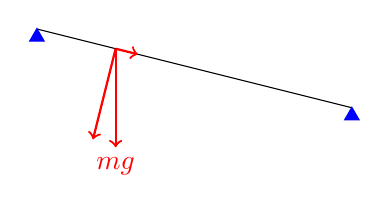
\begin{tikzpicture}
    \draw (-2,1) -- (2,0);
    \node[mark size=3pt,color=blue] at (-2,0.9) {\pgfuseplotmark{triangle*}};
    \node[mark size=3pt,color=blue] at (2,-0.1) {\pgfuseplotmark{triangle*}};
    \draw [->, thick,red] (-1,0.75) -- (-1,-0.5) node[below ]{$mg$};
    \draw [->, thick,red] (-1,0.75) -- (-1+0.28,0.75-0.07);
    \draw [->, thick,red] (-1,0.75) -- (-1-0.25*1.15,0.75-1*1.15);
    \end{tikzpicture}
    \end{center}
    
    \item
    \item
    \item
\end{enumerate}

\subsection{Problem Set 3-1 - 1961 Nov 03 (3.16)}
Direct measurement can be done for the
\begin{itemize}
    \item radius of the earth $R_e=6371\text{km}$
    \item orbital period of the moon $T_M=28\text{d}$
    \item angular diameter of the moon $\delta=30'=0.5^\circ$
    \item earths gravitational acceleration $g=9.81\text{ms}^2$
    \item also Sputnik I orbital data can be looked up $a_\text{satellite}=R_E+584\text{km}$ and $T_\text{satellite}=96.2\text{min}$
    \item height difference between low and high tide $\Delta h=1\text{m}$
\end{itemize}

\begin{enumerate}
\item We use Keplers 3rd law
\begin{align}
    \frac{a_M^3}{T_M^2}&=\frac{a_\text{satellite}^3}{T_\text{satellite}^2}\\
    a_M&=a_\text{sat}\left(\frac{T_M}{T_\text{sat}}\right)^{2/3}
\end{align}
then the radius of the moon is given by
\begin{align}
R_M=\frac{a_M}{2}\tan\delta=\frac{a_\text{sat}}{2}\left(\frac{T_M}{T_\text{sat}}\right)^{2/3}\tan\delta
\end{align}
and the mass by
\begin{align}
    m_M&=\rho_M V_M=\frac{4}{3}\pi\rho_M R_M^3\\
    &=\frac{4}{3}\pi\rho_M \left(\frac{a_\text{sat}}{2}\left(\frac{T_M}{T_\text{sat}}\right)^{2/3}\tan\delta \right)^3\\
    &=\frac{1}{6}\pi\rho_M a_\text{sat}^3\left(\frac{T_M}{T_\text{sat}}\right)^2\tan^3\delta \\
    &\approx\frac{1}{6}\pi\rho_E a_\text{sat}^3\left(\frac{T_M}{T_\text{sat}}\right)^2\tan^3\delta 
\end{align}
where we approximated the moon by the earth mass density. From the gravitational law we can obtain the earth density by
\begin{align}
    g&=\frac{F_g}{m}=\frac{Gm_E}{R_E^2}\quad\rightarrow\quad m_E=\frac{gR_E^2}{G}\\
    \rho_E&=\frac{m_E}{V_E}=\frac{m_E}{\frac{4}{3}\pi R_E^3}=\frac{3g}{4\pi G R_E}.
\end{align}
Therefore the mass of the moon is given by
\begin{align}
    m_M&\approx\frac{g}{ 8G R_E} a_\text{sat}^3\left(\frac{T_M}{T_\text{sat}}\right)^2\tan^3\delta \\
    &=1.16\cdot10^{23}\text{kg}.
\end{align}

\item  We use Keplers 3rd law (for the earth-moon system) and the gravitational law for the earth
\begin{align}
    \frac{a_M^3}{T_M^2}&=\frac{G(m_E+m_M)}{4\pi^2}\approx\frac{Gm_E}{4\pi^2}=\frac{a_\text{satellite}^3}{T_\text{satellite}^2}\\
    g&=\frac{F_g}{m}=\frac{Gm_E}{R_E^2}
\end{align}
and obtain
\begin{align}
    \frac{a_\text{satellite}^3}{T_\text{satellite}^2}&=\frac{gR_E^2+Gm_M}{4\pi^2}\\
    m_M&=\frac{4\pi^2}{G}\left(\frac{a_\text{satellite}^3}{T_\text{satellite}^2}-\frac{gR_E^2}{4\pi^2}\right)\\
    &=7.07\cdot10^{21}\text{kg}.
\end{align}
This result is quite sensitive to the satellite orbital data.


\item We will use the earth tidal data. Lets assume circular orbits with $a_E+a_M=D$ which we can justify by observation (as the moon appears to have constant angular diameter). As reference system we use the center of mass of the system

\begin{center}
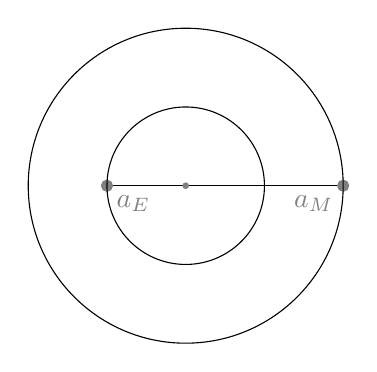
\begin{tikzpicture}
\draw (-1,0) -- (2,0);
\filldraw [gray] (-1,0) circle (2pt) node[below right]{$a_E$};
\filldraw [gray] (2,0) circle (2pt) node[below left]{$a_M$};
\filldraw [gray] (0,0) circle (1pt);
\draw (0,0) circle (2);
\draw (0,0) circle (1);
\end{tikzpicture}
\end{center}
\begin{align}
    m_E\omega^2a_E&=\frac{Gm_Em_M}{D^2}=m_M\omega^2a_M\\
    &\rightarrow a_E=\frac{m_MD}{m_E+m_M}\\
    &\rightarrow \omega^2=\frac{G(m_E+m_M)}{D^3}\\
    &\rightarrow \omega^2a_E^2=\frac{Gm_M^2}{D(m_E+m_M)}\\
    &\rightarrow \frac{R_E}{a_E}=\frac{m_E+m_M}{m_M}\frac{R_E}{D}
\end{align}

\begin{center}
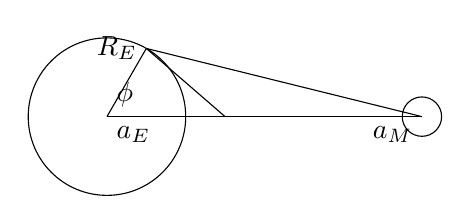
\begin{tikzpicture}
\draw (-2,0) -- (2,0);
\draw (-2,0) circle (1) node[below right]{$a_E$} node[above right]{$\phi$};
\draw (2,0) circle (0.25) node[below left]{$a_M$};
\draw (2,0) -- (-1.5,0.866);
\draw (-2,0) -- (-1.5,0.866) node[left]{$R_E$};
\draw (-0.5,0) -- (-1.5,0.866);
\end{tikzpicture}
\end{center}
The potential is then given by (gravity of moon and earth as well as the centripetal potential around the center of gravity)
\begin{align}
    V&=V_\text{G,moon}+V_\text{G,earth}+V_\text{cent}\\
    &=-\frac{G m_M}{\sqrt{R_E^2+D^2-2DR_E\cos\phi}}-\frac{Gm_E}{R_E}-\frac{1}{2}\omega^2(R_E^2+a_E^2-2a_ER_E\cos\phi)\\
    &=-\frac{Gm_M}{D\sqrt{\left(\frac{R_E}{D}\right)^2+1-2\frac{R_E}{D}\cos\phi}}-\frac{Gm_E}{R_E}-\frac{1}{2}\omega^2a_E^2\left[\left(\frac{R_E}{a_E}\right)^2+1-2\frac{R_E}{a_E}\cos\phi\right]\\
    &\approx-\frac{Gm_M}{D}\left(1+\frac{R_E}{D}\cos\phi+\frac{3}{2}\left(\frac{R_E}{D}\right)^2\cos^2\phi\right)-\frac{Gm_E}{R_E}\\
    &\quad\quad\quad-\frac{1}{2}\omega^2a_E^2\left[\left(\frac{R_E}{a_E}\right)^2+1-2\frac{R_E}{a_E}\cos\phi\right]\\
    &\approx-\frac{Gm_M}{D}\left(1+\frac{R_E}{D}\cos\phi+\frac{3}{2}\left(\frac{R_E}{D}\right)^2\cos^2\phi\right)-\frac{Gm_E}{R_E}\\
    &\quad\quad\quad-\frac{1}{2}\frac{Gm_M^2}{D(m_E+m_M)}\left[\left(\frac{m_E+m_M}{m_M}\frac{R_E}{D}\right)^2+1-2\frac{m_E+m_M}{m_M}\frac{R_E}{D}\cos\phi\right]\\
    &\approx-\frac{Gm_M}{D}-\frac{3Gm_M}{2D}\frac{R_E^2}{D^2}\cos^2\phi-\frac{Gm_E}{R_E}\\
    &\quad\quad\quad-\frac{1}{2}\frac{Gm_M^2}{D(m_E+m_M)}\left[\left(\frac{m_E+m_M}{m_M}\frac{R_E}{D}\right)^2+\frac{m_M^2D^2}{m_M^2D^2}\right]\\
    &\approx-\frac{Gm_M}{D}-\frac{3Gm_M}{2D}\frac{R_E^2}{D^2}\cos^2\phi-\frac{Gm_E}{R_E}-\frac{G}{2}\left[(m_E+m_M)\frac{R_E^2}{D^3}+\frac{m_M^2}{m_E+m_M}\frac{1}{D}\right].
\end{align}
with the angular dependent tidal part
\begin{align}
    V_\text{tidal}&=
    -\frac{3 G R_E^2m_M }{2D^3}\cos ^2\phi.
\end{align}
The tidal water surface would be formed by the the surface $r_\text{surf}(\phi)=R_E+h$ of constant potential. The height difference between low and high tide can then be estimated by 
\begin{align}
   -\frac{3 G R_E^2m_M }{2D^3} 
   &= Gm_E\left(\frac{1}{R_E+h}-\frac{1}{R_E}\right)\\
   &\approx Gm_E\left(\frac{1}{R_E\left(1+\frac{h}{R_E}\right)}-\frac{1}{R_E}\right)\\
   &\approx \frac{Gm_E}{R_E}\left(\left(1-\frac{h}{R_E}\right)-1\right)
\end{align}
which gives
\begin{align}
    h=\frac{3R_E^4}{2D^3}\frac{m_M}{m_E}.
\end{align}
Using the results from above
\begin{align}
    m_E&=\frac{gR_E^2}{G}\\
    \omega^2&=\frac{G(m_E+m_M)}{D^3}\\
    &\quad\rightarrow\quad D^3=\frac{G(m_E+m_M)}{\omega^2}=G(m_E+m_M)\frac{T_M^2}{4\pi^2}
\end{align}
we obtain
\begin{align}
    h=\frac{6\pi^2R_E^4T_M^2}{G(m_E+m_M)T_M^2}\frac{m_M}{m_E}.
\end{align}
and can subsequently solve for $m_M$
\begin{align}
    m_M&=\frac{G h m_E^2 T^2}{6 \pi ^2 R_E^4-G h m_E T^2}\\
    &=\frac{m_E}{\frac{6\pi^2 R_E^4}{G h m_E T^2}-1}\\
    &=\frac{g^2 h T_M^2 R_E^2}{G(6\pi^2R_E^2 -ghT_M^2)}\\
    &=\frac{g R_E^2}{G\left(\frac{6\pi^2R_E^2}{ghT_M^2} -1\right)}\\
    &=1.38\cdot10^{23}\text{kg}
\end{align}
\end{enumerate}

\subsection{Problem Set 3-3 - 1961 Nov 03 (3.10)}
\begin{enumerate}[label=(\alph*)]
\item We use Keplers 3rd law for the earth
\begin{align}
    \frac{a_E^3}{T_E^2}&=\frac{G(m_S+m_E)}{4\pi^2}\approx\frac{Gm_S}{4\pi^2}\\
\end{align}
and the stars $a$ and $b$
\begin{align}
    \frac{a^3}{T^2}&=\frac{G(m_A+m_B)}{4\pi^2}\\
    \frac{(Ra_E)^3}{(TT_E)^2}&=\frac{R^3}{T^2}\frac{a_E^3}{T_E^2}=\frac{R^3}{T^2}\frac{Gm_S}{4\pi^2}=\frac{G(m_A+m_B)}{4\pi^2}\\
    &\rightarrow m_A+m_B = \frac{R^3}{T^2}m_S=\frac{729}{25}m_S
\end{align}

\item For a the circular orbits we have the stability condition
\begin{align}
    m_A\omega^2r_A&=F_{AB}=m_B\omega^2r_B\\
    &\rightarrow m_A\omega v_A=m_B\omega v_B\\
    &\rightarrow \frac{m_A}{m_B} =\frac{v_B}{v_A}=\frac{1}{5}
\end{align}
with $m_B=5m_A$ we have 
\begin{align}
    m_A&=\frac{243}{50}m_S\\
    m_B&=\frac{243}{10}m_S.
\end{align}
\end{enumerate}

\subsection{Book (2.13)}
The resulting force is
\begin{align}
F_r=(\sqrt{2}-1)\cdot 50N
\end{align}
pointing 45 degrees (direction North-East).

To hold the system in place all the sum of the torques must also vanish. We assume that the distance of the point to $O$ is $x$ then the torques regarding $O$ are
\begin{align}
M_O&=0\\
M_P&=0\\
M_Q&=0.1\text{m}\cdot50\text{N}=5\text{N}\\
M_r&=x\cdot\frac{F_r}{\sqrt{2}}=x\frac{\sqrt{2}-1}{\sqrt{2}}50\text{N}\\
&\rightarrow x=\frac{1}{10}\frac{\sqrt{2}}{\sqrt{2}-1}=0.3414\text{m}
\end{align}


\subsection{Book (2.14)}
Energy conservation gives
\begin{align}
W_1D\sin\theta-W_2D\sin\theta&=\frac{1}{2}\frac{W_1}{g}v^2+\frac{1}{2}\frac{W_2}{g}v^2\\
(W_1-W_2)D\sin\theta&=\frac{W_1+W_2}{2g}v^2\\
&\rightarrow v=\sqrt{\frac{2gD\sin\theta(W_1-W_2)}{W_1+W_2}}
\end{align}

\subsection{Book (2.15)}
Energy conservation gives
\begin{align}
WD\sin\phi-WD\sin\theta&=2\frac{1}{2}\frac{W}{g}v^2\\
WD(\sin\phi-\sin\theta)&=\frac{W}{g}v^2\\
&\rightarrow v=\sqrt{gD(\sin\theta-\sin\theta)}
\end{align}

\subsection{Book (2.17)}
Net torque must vanish 
\begin{align}
\left(WL+w\frac{L}{2}\right)\sin\theta=M=Fx
\end{align}
Then split $F$ into $T$ and a force along $x$
\begin{align}
\frac{F}{T}&=\cos\theta\\
T&=\frac{F}{\cos\theta}=\frac{\left(WL+w\frac{L}{2}\right)\sin\theta}{x \cos\theta}=\frac{L}{x}\left(W+\frac{w}{2}\right)\tan\theta
\end{align}




\subsection{Book (2.22)}
The center of the spheres build a tetrahedron
\begin{figure}[!h]
\centering
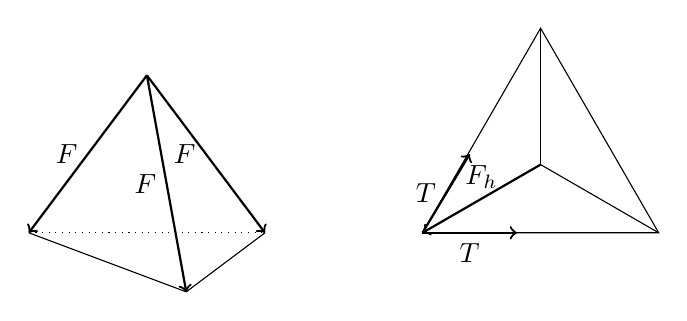
\begin{tikzpicture}
\draw[thick,  <-]  (0,0) -- (1.5,2) node[midway, left] {$F$};
\draw[thick,  ->]  (1.5,2) -- (3,0)node[midway, left] {$F$};
\draw[thick,  <-] (2,-0.75) -- (1.5,2)node[midway, left] {$F$};
\draw[dotted] (0,0) -- (3,0);
\draw (0,0) -- (2,-0.75) -- (3,0);

\draw (5,0) -- (8,0) -- (6.5,0.866*3) -- (5,0);
\draw[thick, <-] (5,0) -- (6.5,0.866)node[midway, above] {$F_h$};
\draw[thick, ->] (5,0) -- (6.2,0)node[midway, below] {$T$};
\draw[thick, ->] (5,0) -- (5.6,1)node[midway, left] {$T$};
\draw (8,0) -- (6.5,0.866);
\draw (6.5,0.866*3) -- (6.5,0.866);
\end{tikzpicture}
\caption{Problem (2.22)}
\end{figure}
where each connection has to carry a third of the weight $mg$
\begin{align}
F=\frac{mg}{3\cos\alpha}
\end{align}
where $\alpha$ is the angle of the edge
\begin{align}
\cos\alpha=\frac{H}{a}=\frac{\sqrt{a^2-\left(\frac{2}{3}h\right)^2}}{a}=\frac{\sqrt{a^2-\left(\frac{2}{3}\frac{\sqrt{3}}{2}a\right)^2}}{a}=\sqrt{2/3}.
\end{align}
The horizontal projection is then
\begin{align}
F_h=F\sin\alpha=\frac{mg}{3}\tan\alpha.
\end{align}
Projecting them in the plane gives
\begin{align}
F_h&=\sqrt{T^2+T^2-2T^2\cos\frac{2\pi}{3}}\\
&\rightarrow T=\frac{mg}{3\sqrt{6}}
\end{align}
including the safety margin we obtain
\begin{align}
\widetilde{T}=3T=\frac{mg}{\sqrt{6}}=2\text{ton-wt}
\end{align}

\subsection{Book (14.7)}
\begin{align}
dV&=2\pi \rho dA\\
&=2\pi (R+r\cos\phi) dA\\
\rightarrow V&=2\pi\int_0^\pi\int_0^R(R+r\cos\phi)r\,dr\,d\phi\\
&=2\pi^2R^3
\end{align}

\subsection{Book (14.8)}
CM is at $R/3$ so $\frac{2}{3}R\cdot M=\frac{1}{3}R\cdot 2M$ then
\begin{align}
J&=J_1+J_2\\
&=M\left(\frac{2}{3}R\right)^2+2M\left(\frac{1}{3}R\right)^2\\
&=\frac{4+2}{9}MR^2=\frac{2}{3}MR^2
\end{align}
and
\begin{align}
T=\frac{1}{2}J\omega^2=\frac{1}{3}MR^2\omega^2
\end{align}

\subsection{Book (14.10)}
Consider two discs - the big one and the small one (the hole - with negative area mass density) - the combination/superposition makes up the disc with the hole
\begin{align}
m_1&=\rho_A\pi R^2\\
m_2&=-\rho_A\pi (R/2)^2
\end{align}
then the CM
\begin{align}
m_1x&=(R/2-x)m_2\\
\rightarrow x
&=\frac{m_2R/2}{m_1+m_2}
=\frac{-(R/2)^3}{R^2-(R/2)^2}
=-\frac{\frac{R^3}{8}}{\frac{3}{4}R^2}=-\frac{1}{6}R\approx 1.66\text{cm}
\end{align}



\subsection{Problem Set 3-4 - 1961 Nov 03 (?.??)}
\begin{align}
    g_M=\frac{GM_M}{R_M^2}&=\frac{4}{3}G\rho_M R_M=\frac{4}{3}G (0.537\rho_E) (0.716R_E)=0.384 \cdot g_E
\end{align}

\subsection{Problem Set 1a 4-1 - 1961 Nov 10 (11.16)}
For the masses we obtain
\begin{align}
\widetilde{m}_i
&=\rho_i V_i=\frac{4}{3}\pi (kR_i)^3\rho_i\\
&=k^3m_i
\end{align}
The third Kepler law is given by
\begin{align}
T^2=a^3\frac{4\pi}{G(M+m)}
\end{align}
applying the scaling to $a$ we have $\widetilde{a}^3=(ka)^3$ and therefore
\begin{align}
\widetilde{T}^2
&=\widetilde{a}^3\frac{4\pi}{G(\widetilde{M}+\widetilde{m})}\\
&=k^3a^3\frac{4\pi}{G(k^3M+k^3m)}\\
&=a^3\frac{4\pi}{G(M+m)}\\
&=T^2.
\end{align}
So we conclude that there is no change in $T$. 

\subsection{Problem Set 1a 4-3 - 1961 Nov 10 (??.??)}
With $\vec{a}=(1,0,2)$ and $\vec{b}=(1,4,0)$
\begin{align}
\cos\alpha=\frac{\vec{a}\cdot\vec{b}}{|\vec{a}|\,|\vec{b}|}
=1/\sqrt{85}
\end{align}

\subsection{Problem Set 1a 4-6 - 1961 Nov 10 (??.??)}
The 3, 4, 5 triangle is rectangular with and incline angle $\alpha$
\begin{align}
\sin\alpha&=3/5\\
\cos\alpha&=4/5
\end{align}
and therefore
\begin{align}
F_{A,\parallel}&=M_Ag(\sin\alpha-\mu_A\cos\alpha)\\
F_{B,\parallel}&=M_Bg(\sin\alpha-\mu_B\cos\alpha)
\end{align}
(a) Then
\begin{align}
a
&=\frac{F_{A,\parallel}+F_{B,\parallel}}{M_A+M_B}\\
&=\frac{M_A(\sin\alpha-\mu_A\cos\alpha)+M_B(\sin\alpha-\mu_B\cos\alpha)}{M_A+M_B}g\\
&=\frac{(M_A+M_B)\sin\alpha-(M_A\mu_A+M_B\mu_B)\cos\alpha}{M_A+M_B}g\\
&=\left(\sin\alpha-\frac{M_A\mu_A+M_B\mu_B}{M_A+M_B}\cos\alpha\right)g\\
&=4.84\text{m/s}^2
\end{align}
(b) Newton 3
\begin{align}
F_{A,\parallel}-M_Aa&=T\\
F_{B,\parallel}-M_Ba&=-T
\end{align}
then
\begin{align}
2T
&=(F_{A,\parallel}-F_{B,\parallel})-(M_A-M_B)a\\
T&=\frac{M_AM_B}{M_A+M_B}(\mu_B-\mu_A)g\cos\alpha\\
&=2.09\text{N}
\end{align}


\subsection{Problem Set 1a 6-1 - 1961 Dec 01 (12.7)}
The general spacial part of the 4-acceleration is given by
\begin{align}
\frac{d^2x^k}{d\tau^2}
&=a^k\gamma^2+u^k\gamma^4(\vec{u}\cdot\vec{a})\frac{1}{c^2}
\end{align}
and simplifies in 1 dimension to
\begin{align}
\frac{d^2x}{d\tau^2}
&=a\gamma^2+\frac{av^2}{c^2}\gamma^4\\
&=a\gamma^2\left(1+\frac{v^2}{c^2}\gamma^2\right)\\
&=a\gamma^2\left(\frac{1-v^2/c^2}{1-v^2/c^2}+\frac{v^2/c^2}{1-v^2/c^2}\right)\\
&=a\gamma^2\frac{1}{1-v^2/c^2}\\
&=\frac{a}{[1-v^2/c^2]^2}
\end{align}
with Newtons 3rd law
\begin{align}
m_0\frac{d^2x^\mu}{d\tau^2}=f^\mu=\gamma(\vec{F},\frac{1}{c}\vec{F}\cdot\vec{u})
\end{align}
we have
\begin{align}
m_0\frac{a}{[1-v^2/c^2]^2}&=\frac{F}{\sqrt{1-\frac{v^2}{c^2}}}\\
m_0\frac{a}{[1-v^2/c^2]^{3/2}}&=F
\end{align}
Now lets calculate $v$ and $a$
\begin{align}
v&=\frac{dx}{dt}=\frac{c^2t}{\sqrt{b^2+c^2t^2}}\quad\rightarrow\quad t=\frac{bv}{c^2\sqrt{1-v^2/c^2}}\\
a&=\frac{d^2x}{dt^2}=\frac{b^2c^2}{(b^2+c^2t^2)^{3/2}}\\
&=\frac{c^2}{b}(1-v^2/c^2)^{3/2}
\end{align}
and we see $F=m_0c^2/b$.

\subsection{Problem Set 1a 6-6 - 1961 Dec 01 (12.8)}
\begin{enumerate}[a)]
\item
\begin{align}
\Delta m=\frac{W}{c^2}=30.12\text{kg}
\end{align}

\item Step by step - one heavy water molecule contains to deuterium atoms
\begin{align}
\dot{m}&=\frac{\Delta m}{T}\\
\dot{N}_{D_2O}&=\frac{\dot{m}}{(M_{He^4}-2M_{H^2})u}\\
\dot{n}_{D2O}&=\frac{\dot{N}_{D_2O}}{N_A}\\
\dot{m}_{D2O}&=\dot{n}_{D_2O}M_{D_2O}\\
&=\frac{WM_{D_2O}}{(M_{He^4}-2M_{H^2})uTc^2N_A}\\
&=0.75\text{g}
\end{align}
\end{enumerate}

\subsection{Problem Set 1b 3-3 - 1962 Jan 16 (??.??)}
\begin{enumerate}
    \item 
    \item For the angular momentum (without precision) we get
    \begin{align}
        L=J\omega=\frac{1}{2}MR^2\omega
    \end{align}
    \item With a little geometry we see
    \begin{align}
        \frac{d\vec{L}}{dt}&=\vec{a}\times\vec{M}=M\vec{a}\times\vec{g}\\
        \frac{dL}{L}&=\sin d\phi\approx d\phi\\
        &\rightarrow\Omega_1=\frac{d\phi}{dt}=\frac{Mag}{L}=\frac{2ag}{R^2\omega}\\
        &\rightarrow\omega=\frac{2ag}{R^2\Omega_1}
    \end{align}
    \item
\end{enumerate}

\subsection{Problem Set 1b 8-1 - 1962 Nov 19 (48.3)}
In cylinder coordinates
\begin{align}
\nabla\times\mathbf{H}=\mathbf{j}+\dot{\mathbf{D}}\\
\rightarrow\frac{1}{\mu_r\mu_0}\nabla\times\mathbf{B}=\mathbf{j}\\
\rightarrow\frac{1}{\mu_r\mu_0}\oint \mathbf{B}\,d\mathbf{s}=\int\mathbf{j}\,d\mathbf{A}\\
\rightarrow\frac{1}{\mu_r\mu_0}2\pi r B_\varphi(r)=I_\text{inside}\\
\rightarrow B_\varphi(r)=\frac{\mu_r\mu_0I_\text{inside}}{2\pi r}
\end{align}
$B_r,B_z=0$
\begin{enumerate}[(a)]
\item
\begin{align}
B_\varphi=\frac{\mu_r\mu_0I\frac{r^2}{a^2}}{2\pi r }=\frac{\mu_r\mu_0I}{2\pi}\frac{r}{a^2}
\end{align}
\item
\begin{align}
B_\varphi=\frac{\mu_r\mu_0I}{2\pi}\frac{1}{r}
\end{align}
\item
\begin{align}
B_\varphi&=\frac{\mu_r\mu_0I}{2\pi}\frac{1}{r}-\frac{\mu_r\mu_0I}{2\pi}\frac{1}{r}\frac{r^2-b^2}{c^2-b^2}\\
&=\frac{\mu_r\mu_0I}{2\pi}\frac{1}{r}\frac{r^2-c^2}{b^2-c^2}
\end{align}
\item
\begin{align}
B_\varphi=0
\end{align}
\end{enumerate}

\subsection{Problem Set 1b 8-4 - 1962 Nov 19 (49.2)}
With $d^3r' \mathbf{j}(\mathbf{x'})=I\,d\mathbf{s}'$ we see
\begin{align}
\mathbf{A}(\mathbf{x})
&=\frac{\mu_0}{4\pi}\int d^3r'\frac{\mathbf{j}(\mathbf{x'})}{|\mathbf{x}-\mathbf{x}'|}\\
&=\frac{\mu_0}{4\pi}I\int d\mathbf{s}'\frac{1}{|\mathbf{x}-\mathbf{x}'|}
\end{align}
now we apply to the problem
\begin{align}
\mathbf{A}(\mathbf{x})
&=\frac{\mu_0}{4\pi}I\left[\mathbf{e}_z\int_{-\infty}^{-R} dz'\frac{1}{|z'|}+\mathbf{e}_\varphi\int_0^\pi R\,d\varphi'\frac{1}{R}+\mathbf{e}_z\int^\infty_R dz'\frac{1}{|z'|}\right]\\
&=\frac{\mu_0I}{4}\mathbf{e}_\varphi
\end{align}
Then
\begin{align}
\mathbf{B}&=\nabla\times\mathbf{A}\\
&=-\frac{\partial A_\varphi}{\partial z}\mathbf{e}_r+0\,\mathbf{e}_\varphi+\frac{1}{r}\frac{\partial (rA_\varphi)}{\partial r}\mathbf{e}_z\\
&=\frac{\mu_0I}{4r}\mathbf{e_z}
\end{align}

\subsection{Problem Set 1b 11-1 - 1962 Feb 16 (20.11)}

\begin{figure}[!h]
\begin{center}
\usetikzlibrary{quotes,angles}
\begin{tikzpicture}
\draw[thick,->] (0,0) -- (4.5,0);
\draw[thick,->] (0,0) -- (0,2.5);
\draw[thick] (1.3,2) arc (110:210:2cm);
\draw (-1,1.5) -- (0.5,1.5) -- (4,0);
\draw[dashed] (-0.5,2.5) -- (0.5,1.5) -- (2,0);

\draw (-1,1.5) coordinate (a)  (0.5,1.5) coordinate (b)  (-0.5,2.5) coordinate (c)
pic["$\alpha$", draw=orange, <->, angle eccentricity=1.2, angle radius=0.8cm] {angle=c--b--a};

\draw (2,0) coordinate (a)  (0.5,1.5) coordinate (b)  (4,0) coordinate (c)
pic["$\beta$", draw=orange, <->, angle eccentricity=1.2, angle radius=0.8cm] {angle=a--b--c};

\draw (0.5,1.5) coordinate (a)  (2,0) coordinate (b)  (4,0) coordinate (c)
pic["$\pi-\alpha$", draw=orange, <->, angle eccentricity=1.2, angle radius=0.4cm] {angle=c--b--a};

\draw[dashed] (0,1) -- (0.5,1.5) -- (1.5,2.5);
\draw[dotted]  (0.5,1.5) -- (3,1.5);
\draw (1.5,2.5) coordinate (a)  (0.5,1.5) coordinate (b)  (3,1.5) coordinate (c)
pic["$\gamma$", draw=orange, <->, angle eccentricity=1.2, angle radius=0.8cm] {angle=c--b--a};


\draw (0.5,1.5) -- (4,0) node[midway, anchor=south west] {$\sqrt{y^2+(F-x)^2}$};
\draw[orange, thick] (0.0,0) -- (0.5,0) node[midway, below] {$x$};
\draw[purple, thick] (0.5,0) -- (2,0) node[midway, below] {$z$};
\draw[red, thick] (2,0) -- (4,0) node[midway, below] {$F-x-z$};
\draw[blue, thick] (0.5,0) -- (0.5,1.5) node[midway, left] {$y$};
\end{tikzpicture}
\end{center}
\caption{Problem (20.11)}
\end{figure}

We start with Snell's law
\begin{align}
\sin\alpha=n\sin\beta
\end{align}
and the sine law
\begin{align}
\frac{\sin(\pi-\alpha)}{\sqrt{y^2+(F-x)^2}}&=\frac{\sin\beta}{F-x-z}
\end{align}
we also see
\begin{align}
\frac{y}{z}=\tan\alpha
\end{align}
most importantly we have for the slope of the surface
\begin{align}
\frac{dy}{dx}&=\tan\gamma\\
&=\tan\left(\pi/2-\alpha\right)=\cot\alpha=\frac{1}{\tan\alpha}
\end{align}
Now we can put it all together
\begin{align}
\frac{\sin(\alpha)}{\sqrt{y^2+(F-x)^2}}&=\frac{\sin\alpha}{n(F-x-
\frac{y}{\tan\alpha})}\\
\frac{1}{\sqrt{y^2+(F-x)^2}}&=\frac{1}{n[(F-x)-
y\frac{dy}{dx}]}\\
(F-x)-y\frac{dy}{dx}&=\frac{1}{n}\sqrt{y^2+(F-x)^2}
\end{align}
The ODE can be solved by Mathematica which gives two solutions
\begin{align}
y_1&=\pm\sqrt{2Fx\left(1-\frac{1}{n}\right)-\left(1-\frac{1}{n^2}\right)x^2}\\
y_2&=\pm\sqrt{2Fx\left(1+\frac{1}{n}\right)-\left(1-\frac{1}{n^2}\right)x^2}
\end{align}
\iftoggle{includeCoverPic}{
\begin{figure}[h]
\centering
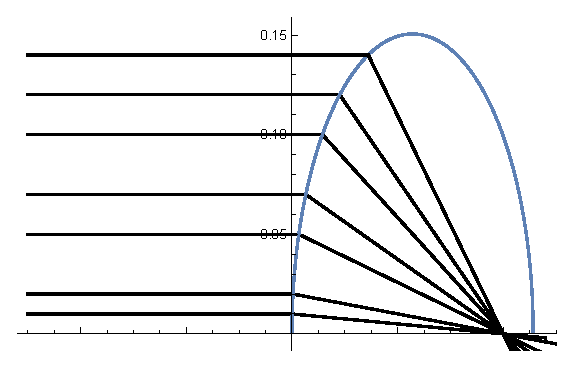
\includegraphics[scale=0.4]{Feynman2011.eps}
\caption{Light rays for solution $y_1$ of Feynman problem (20.11)}
\end{figure}
}

\subsection{Book (20.14)}
Using the sine law for the appropriate triangle inside the sphere (cosine law to calculate the length of one side) we obtain
\begin{align}
\frac{\sin\beta}{R}&=\frac{\sin\alpha}{\sqrt{R^2+R^2-2R\cdot R\cos\alpha}}\\
\frac{\sin\alpha}{nR}&=\frac{\sin\alpha}{\sqrt{2}R\sqrt{1-\cdot R\cos\alpha}}
\end{align}
where we used Snells law. Simplifying further
\begin{align}
\cos\alpha&=1-\frac{n^2}{2}\\
\sqrt{1-\sin^2\alpha}&=1-\frac{n^2}{2}\\
\sin^2\alpha&=1-\left(1-\frac{n^2}{2}\right)^2\\
\frac{y^2}{4R^2}&=1-\left(1-\frac{n^2}{2}\right)^2\\
&\rightarrow y=2nR\sqrt{1-\frac{n^2}{4}}=1.92R
\end{align}

\subsection{Book (20.16)}
First lens
\begin{align}
\frac{1}{f}&=\frac{1}{g}+\frac{1}{b}\quad\rightarrow\quad b=\frac{gF}{g-F}\\
\frac{B}{G}&=\frac{b}{g}\quad\rightarrow\quad B=G\frac{b}{g}=\frac{G}{g}\frac{gF}{g-F}
\end{align}
Distant object means
\begin{align}
B\simeq\frac{GF}{g}
\end{align}
The second lens works as a magnifying glass - focussing at infinity means the virtual picture is at infinity and therefore the object (real picture of the first lens) needs to be at the focus of the second lens.
The angle is then given by
\begin{align}
\tan\alpha'=\frac{B}{f}=\frac{GF}{gf}
\end{align}
without lenses the angle would have been
\begin{align}
\tan\alpha=\frac{G}{g}.
\end{align}
Then
\begin{align}
M=\tan\alpha'/\tan\alpha=F/f.
\end{align}

\subsection{Book (20.19)}
First lens
\begin{align}
\frac{1}{f_1}&=\frac{1}{g}+\frac{1}{b}\\
&\rightarrow b=\frac{gf_1}{g-f_1}=\frac{30,000}{970}\text{cm}=30.93\text{cm}
\end{align}
so real picture of first lens would be
\begin{align}
30.93\text{cm}-27.50\text{cm}=3.43\text{cm}
\end{align}
right of second lens. 

\subsection{Book (20.20) - NOT DONE YET}
The geometry of the system is
\begin{align}
x^2+y^2&=l^2\\
x&=l\cos\alpha\\
y&=l\sin\alpha.
\end{align}
The vertical heights of the endpoints are then
\begin{align}
h_\text{left}
&=x\sin 60=\frac{\sqrt{3}}{2}x=\frac{\sqrt{3}}{2}l\cos\alpha\\
h_\text{right}&=y\sin 30=\frac{1}{2}y=\frac{1}{2}l\sin\alpha.
\end{align}
Height of the center of gravity
\begin{align}
h_S
&=\frac{h_\text{left}+h_\text{right}}{2}\\
&=\frac{\sqrt{3}\cos\alpha+1\sqrt{1-\cos^2\alpha}}{4}l\\
&=\frac{\epsilon\cos\alpha+1\sqrt{1-\epsilon^2}}{4}l
\end{align}
Stability condition: center of gravity in lowest position. So
\begin{align}
\frac{d}{d\epsilon}h_s(\epsilon)=0\quad&\rightarrow\quad\epsilon=\sqrt{3}/2\\
&\rightarrow\quad\alpha=30^o
\end{align}

\subsection{Problem Set 1b  15-1 - 1962 March 6 (19.35)}
We start with
\begin{align}
m\ddot{x}+kx+\alpha\dddot{x}&=qE_0\cos\omega t\\
\end{align}
the are only interested in the stationary part of the solution (after initial conditions are damped away). So we assume
\begin{align}
x(t)=A\cos(\omega t+\delta)
\end{align}
Substituting gives
\begin{align}
(A(k-m\omega^2)\cos\delta+A\alpha\omega^3\sin\delta-qE_0)\cos\omega t+A((m\omega^2-k)\sin\delta+\alpha\omega^3\cos\delta)\sin\omega t=0
\end{align}
which requires
\begin{align}
(m\omega^2-k)\sin\delta+\alpha\omega^3\cos\delta)&=0\\
A(k-m\omega^2)\cos\delta+A\alpha\omega^3\sin\delta-qE_0&=0\\
\rightarrow \tan\delta&=\frac{\alpha\omega^3}{k-m\omega^2}\\
\rightarrow A&=\frac{qE_0}{\sqrt{(k-m\omega^2)^2+\alpha^2\omega^6}}
\end{align}



\subsection{Problem Set 1b  15-2 - 1962 March 6 (?.??)}
Lets derive the Lambert-Beer Law
\begin{align}
\Delta I
&=-I \frac{N\sigma}{dy\cdot dz}\\
&=-I \frac{N\sigma\cdot dx}{dy\cdot dz\cdot dx}\\
\frac{\Delta I}{dx}&=-I\frac{N\sigma}{V}\\
I'&=-I\frac{N\sigma}{V}
\end{align}
then
\begin{align}
I(x)=I_0e^{-\frac{N\sigma}{V}x}
\end{align}


\subsection{Problem Set 1c 13-1 - 1962 May 25 (?.??)}
We cheat a little and use the Lagrange formalism 
\begin{align}
L&=T-V\\
&=\frac{m_1}{2}\dot{x}^2+\frac{m_2}{2}\dot{y}^2-\frac{k_1}{2}x^2-\frac{k_2}{2}y^2-\frac{k}{2}(x-y)^2
\end{align}
then
\begin{align}
\frac{\partial L}{\partial x_i}-\frac{d}{dt}\frac{\partial L}{\partial\dot{x}_i}=0
\end{align}
gives
\begin{align}
m_1\ddot{x}+k_1x+k(x-y)=0\quad\rightarrow\quad \ddot{x}+\omega_0^2x+\frac{k}{m_1}(x-y)=0\\
m_2\ddot{y}+k_2y-k(x-y)=0\quad\rightarrow\quad \ddot{y}+\omega_0^2y+\frac{k}{m_2}(y-x)=0
\end{align}


\subsection{Problem Set 1c  13-2 - 1962 May 25 (?.??)}
We obtain
\begin{align}
-A\omega^2+A\omega_0^2+\frac{k}{m_1}(A-B)=0\\
-B\omega^2+B\omega_0^2+\frac{k}{m_2}(B-A)=0
\end{align}
and therefore
\begin{align}
\omega^2=\omega_0^2+\frac{k}{m_1}(1-B/A)\\
\omega^2=\omega_0^2+\frac{k}{m_2}(1-A/B)
\end{align}
both expressions give the same valuers for $\omega$ if
\begin{align}
A/B=1\quad&\rightarrow\quad \omega=\omega_0\\
A/B=-m_2/m_1\quad&\rightarrow\quad \omega=\sqrt{\omega_0+\frac{k}{m_1}+\frac{k}{m_2}}
\end{align} 

\subsection{Problem Set 2a  7-1 - 1962 Nov 12 (46.2)}
Assuming a linear response
\begin{align}
D&=\epsilon_0E+P\\
&=\epsilon_r\epsilon_0E\\
&=\epsilon_0E+(\epsilon_r-1)\epsilon_0E\\
\rightarrow P&=(\epsilon_r-1)\epsilon_0E
\end{align}
$P$ has unites As/m$^2$=Asm/$m^3$ - so it's a dipole volume density. Then
\begin{align}
(\epsilon_r-1)\epsilon_0E&=P=\frac{p_D}{V}=\frac{p_Dp}{N_Ak_BT}\\
\rightarrow p_D^{molecule}=\frac{p_D}{N_A}&=\frac{(\epsilon_r-1)\epsilon_0Ek_BT}{p}\\
&=2.46\cdot10^{-36}\text{Asm}
\end{align}
where we used $E=100$V/m.


\subsection{Problem Set 2a  7-3 - 1962 Nov 12 (47.2)}
Using the Fourier equation (utilising spherical symmetry)
\begin{align}
\frac{Q}{\Delta t}
&=-\lambda\cdot 4\pi a^2\frac{T_\text{univ}-T_\text{core}}{R_E-a}\\
\rightarrow a
&=\frac{Q\left(1\pm\sqrt{1-16\pi R_E\lambda Q^{-1}\Delta t(T_\text{univ}-T_\text{core})}\right)}{8\pi\lambda\Delta t(T_\text{univ}-T_\text{core})}\\
&=6,212\text{km}
\end{align}


\subsection{Problem Set 2b  19-1 - 1963 Mar 35 (??.?)}
\begin{align}
\frac{1}{4\pi\epsilon_0}\frac{qQ}{r^2}+qvB=m\frac{v^2}{r}
\end{align}

\section{{\sc Gershenfeld} - The Nature of Mathematical Modelling}
\subsection{Problem 2.1}
\begin{enumerate}[(a)]
\item 
\begin{align}
V(x)&=V_0+V_1x+V_2x^2+...\\
&\rightarrow V_1=0\\
&\rightarrow F=-\nabla V=2V_2x=kx
\end{align}
\item $x(t)=e^{ft}$
\begin{align}
(mf^2+\gamma f+k)e^{ft}=0\\
f=-\frac{\gamma}{2m}\pm\sqrt{\frac{\gamma^2}{4m^2}-\frac{k}{m}}
\end{align}
\item ???
\end{enumerate}



\section{{\sc Gershenfeld} - The Physics of Information Technology}
\subsection{Problem 2.1}
(a) $10^{-24}\cdot6.6\cdot10^{23}\simeq1$\\
(b) $10^{-9}\cdot100\cdot365\cdot24\cdot60\cdot60\,\text{sec}\simeq3.15\,\text{sec}$
\subsection{Problem 2.2}
With $1\,\text{TB}=10^9\,\text{MB}$
\begin{align}
\frac{10^{9}\,\text{MB}}{\frac{1\,\text{MB}}{3\,\text{mm}}}
=10^{9}\cdot0.003\,\text{m}=3000\,\text{m}
\end{align}



\section{{\sc Weinberg} - Foundation of Modern Physics}

\subsection{Problem 6 - Power of Carnot AC}
\begin{align}
P_\text{therm}&=10\text{kW}\\
\eta&=1-\frac{293}{313}=0.064\\
P&=\frac{P_\text{therm}}{\eta}=156.5\text{kW}
\end{align}


\subsection{Problem 7 - Electrolysis of water}
For each O$_2$ molecule 4 elementary charges are needed (because O$^{2-}$)
\begin{align}
I&=\frac{\Delta Q}{\Delta t}=e\frac{N_e}{\Delta t}\\
m_{O_2}
&=\frac{N_e}{2\cdot 2}M_{O_2}\cdot u\\
&=\frac{I\cdot\Delta t}{4e}M_{O_2}\cdot u\\
\Delta t&=\frac{4em_{O_2}}{IM_{O_2}u}=3,000\,\text{s}
\end{align}





\section{{\sc Thorne, Blandford} - Modern Classical Physics}
\subsection{Exercise 1.1 Practice: Energy Change for Charged Particle}
With $E=p^2/2m$ and (1.7c) we obtain
\begin{align}
    \frac{dE}{dt}&=\frac{d}{dt}\frac{p^2}{2m}=\frac{2 \vec{p}\cdot d\vec{p}/dt}{2m}\\
    &=\frac{q}{m}\vec{p}\cdot (\vec{E}+\vec{v}\times\vec{B})\\
    &=q\vec{v}\cdot (\vec{E}+\vec{v}\times\vec{B})\\
    &=q\vec{v}\cdot\vec{E}.
\end{align}
As $\vec{v}\times\vec{B}$ is orthogonal to $\vec{v}$ (and $\vec{B}$) the scalar product $\vec{v}\cdot(\vec{v}\times\vec{B})$ vanishes.

\subsection{Exercise 1.2 Practice: Particle Moving in a Circular Orbit}
\begin{enumerate}[label=(\alph*)]
\item With
\begin{align}
    \frac{d\vec{n}}{ds}
    =\frac{\vec{n}'-\vec{n}}{R\cdot d\phi}=\frac{\vec{v}'-\vec{v}}{vR\cdot d\phi}
\end{align}
we can calculate the norm
\begin{align}
    \left|\frac{d\vec{n}}{ds}\right|
    &=\frac{\sqrt{v^2+v^2-2v^2\cos(d\phi)}}{vR\cdot d\phi}
    =\frac{v\sqrt{1-\cos(d\phi)}}{vR\cdot d\phi}
    = \frac{v\sqrt{2[1-\cos(d\phi)]}}{vR\cdot d\phi}\\
    &\approx\frac{vd\phi}{vR\cdot d\phi}=\frac{1}{R}
\end{align}
and the scalar product
\begin{align}
    \frac{d\vec{n}}{ds}\cdot\vec{n}
    &=\frac{\vec{n}'\cdot\vec{n}-\vec{n}\cdot\vec{n}}{R\cdot d\phi}=\frac{n^2\cos(d\phi)-n^2}{vR\cdot d\phi}\\
    &\approx \frac{(1-d\phi^2/2)-1}{vR\cdot d\phi}=\frac{d\phi}{2vR}
\end{align}
which vanished for $d\phi\rightarrow0$ and therefore implies that $d\vec{n}$ is orthogonal to $\vec{n}$ (and therefore points to the center).
\item From (a) we know
\begin{align}
    \vec{R}=R^2\frac{d\vec{n}}{ds}
    =R^2\frac{d\vec{v}}{v\cdot ds}
    =R^2\frac{d\vec{v}}{v\cdot ds}
    =\frac{R^2}{v}\frac{d\vec{v}}{dt}\frac{dt}{ds}
    =\left(\frac{R}{v}\right)^2\vec{a}
\end{align}
Taking the absolute value we have
\begin{align}
    R=\frac{R^2}{v^2}a\quad\rightarrow\quad R=\frac{v^2}{a}
\end{align}
and therefore
\begin{align}
    \vec{R}=\frac{R^2}{v^2}\vec{a}=\frac{v^4}{v^2 a^2}\vec{a}=\left(\frac{v}{a}\right)^2\vec{a}.
\end{align}
\end{enumerate}

\subsection{Exercise 1.3 Derivation: Component Manipulation Rules}
\begin{enumerate}
\item (1.9g I) - using (1.9b), (1.9a) and (1.9c)
\begin{align}
    \mathbf{A}\cdot\mathbf{B}
    =(A_j\mathbf{e}_j)\cdot(B_k\mathbf{e}_k)
    =A_jB_k\mathbf{e}_j\cdot\mathbf{e}_k
    =A_jB_k\delta_{jk}
    =A_jB_j
\end{align}
\item (1.9g II) - using (1.9d) and (1.5a)
\begin{align}
    \mathbf{T}&=T_{ijk}\mathbf{e}_i\otimes\mathbf{e}_j\otimes\mathbf{e}_k\\
    \mathbf{T}(\mathbf{A},\mathbf{B},\mathbf{C})
    &=T_{ijk}\mathbf{e}_i\otimes\mathbf{e}_j\otimes\mathbf{e}_k(\mathbf{A},\mathbf{B},\mathbf{C})\\
    &=T_{ijk}(\mathbf{A}\cdot\mathbf{e}_i)(\mathbf{B}\cdot\mathbf{e}_j)(\mathbf{C}\cdot\mathbf{e}_k)\\
    &=T_{ijk}A_iB_jC_k
\end{align}
\item (1.9h) - using (1.9d), (1.6b), (1.9a) and (1.5a)
\begin{align}
    \mathbf{R}
    &=R_{abcd}\mathbf{e}_a\otimes\mathbf{e}_b\otimes\mathbf{e}_c\otimes\mathbf{e}_d\\
    \text{1\&3 contraction}(\mathbf{R})
    &=R_{abcd}(\mathbf{e}_a\cdot\mathbf{e}_c) \mathbf{e}_b\otimes\mathbf{e}_d\\
    &=R_{abcd}\delta_{ac} \mathbf{e}_b\otimes\mathbf{e}_d\\
    &=R_{abad}\mathbf{e}_b\otimes\mathbf{e}_d\\
    \text{components of [1\&3 contraction}(\mathbf{R})]&=R_{abad}\mathbf{e}_b\otimes\mathbf{e}_d(\mathbf{e}_j,\mathbf{e}_k)\\
    &=R_{abad}(\mathbf{e}_b\cdot\mathbf{e}_j)(\mathbf{e}_d\cdot\mathbf{e}_k)\\
    &=R_{abad}\delta_{bj}\delta_{dk}\\
    &=R_{ajak}
\end{align}
\end{enumerate}

\subsection{Exercise 1.4 Example and Practice: Numerics of Component Manipulations}
\begin{align}
    \mathbf{C}
    &=\mathbf{S}(\mathbf{A},\mathbf{B},\_)\\
    &=S_{ijk}\mathbf{e}_i\otimes\mathbf{e}_j\otimes\mathbf{e}_k(\mathbf{A},\mathbf{B},\_)\\
    &=S_{ijk}(\mathbf{A}\cdot\mathbf{e}_i)(\mathbf{B}\cdot\mathbf{e}_j)\mathbf{e}_k\\
    &=S_{ijk}A_iB_j\mathbf{e}_k
\end{align}
\begin{align}
    C_k&=S_{11k}A_1B_1+S_{12k}A_1B_2\\
    C_1&=0,\quad C_2=0,\quad C_3=S_{123}A_1B_2=15
\end{align}
\begin{align}
    \mathbf{D}
    &=\mathbf{S}(\mathbf{A},\_,\mathbf{B})\\
    &=S_{ijk}\mathbf{e}_i\otimes\mathbf{e}_j\otimes\mathbf{e}_k(\mathbf{A},\_,\mathbf{B})\\
    &=S_{ijk}(\mathbf{A}\cdot\mathbf{e}_i)(\mathbf{B}\cdot\mathbf{e}_k)\mathbf{e}_j\\
    &=S_{ijk}A_iB_k\mathbf{e}_j
\end{align}
\begin{align}
    D_j&=S_{1j1}A_1B_1 + S_{1j2}A_1B_2=0
\end{align}
\begin{align}
    \mathbf{W}
    &=\mathbf{A}\otimes\mathbf{B}\\
    &=(A_i\mathbf{e}_i)\otimes(B_j\mathbf{e}_j)\\
    &=A_iB_j \mathbf{e}_i\otimes\mathbf{e}_j
\end{align}
\begin{align}
    W_{11}=12,\quad W_{12}=15,\quad 
\end{align}

\subsection{Exercise 1.5 Practice: Meaning of Slot-Naming Index Notation}
\begin{enumerate}[label=(\alph*)]
\item Somewhat guessing
\begin{align}
    A_iB_{jk}
    &\rightarrow A_iB_{jk}\mathbf{e}_i\otimes\mathbf{e}_j\otimes\mathbf{e}_k\\
    &= (A_i\mathbf{e}_i)\otimes (B_{jk}\mathbf{e}_j\otimes\mathbf{e}_k)\\
    &=A(\_)\otimes B(\_,\_)
\end{align}
\begin{align}
    A_iB_{ji}
    &\rightarrow A_iB_{ji}\mathbf{e}_j\\
    &=(\mathbf{A}\cdot\mathbf{e}_i)B_{ji}\mathbf{e}_j\\
    &=B_{ji}\mathbf{e}_j\otimes\mathbf{e}_i(\_,\mathbf{A})\\
    &=\mathbf{B}(\_,\mathbf{A})
\end{align}
\begin{align}
    S_{ijk}
    &=S_{kji}\rightarrow ...
\end{align}
\begin{align}
    A_iB_i&=AiB_jg_{ij}\rightarrow \mathbf{A}\cdot\mathbf{B}=\mathbf{g}(\mathbf{A},\mathbf{B})
\end{align}

\item Applying the standard machinery
\begin{align}
    \mathbf{T}(\_,\_,\mathbf{A})
    &=T_{ijk}\mathbf{e}_i\otimes\mathbf{e}_j(\mathbf{A}\cdot\mathbf{e}_k)\\
    &=T_{ijk}A_k\mathbf{e}_i\otimes\mathbf{e}_j\\
    &\rightarrow T_{ijk}A_k
\end{align}
\begin{align}
    \mathbf{S}(\mathbf{B},\_)
    &=S_{ab}(\mathbf{B}\cdot\mathbf{e}_a)\mathbf{e}_b\\
    &=S_{ab}B_a\mathbf{e}_b\\
    \mathbf{T}(\_,\mathbf{S}(\mathbf{B},\_),\_)
    &=T_{ijk}\mathbf{e}_i\otimes\mathbf{e}_k(S_{ab}B_a\mathbf{e}_b\cdot\mathbf{e}_j)\\
    &=T_{ijk}\mathbf{e}_i\otimes\mathbf{e}_k(S_{ab}B_a\delta_{bj})\\
    &=T_{ijk}S_{aj}B_a\mathbf{e}_i\otimes\mathbf{e}_k\\
    &\rightarrow T_{ijk}S_{aj}
\end{align}
\end{enumerate}





\subsection{Exercise 1.15 Practice: Geometrized Units}
\begin{enumerate}[label=(\alph*)]
\item $t_P=\sqrt{G\hbar}\quad\rightarrow\quad\sqrt{\frac{G\hbar}{c^5}}= 5.39\cdot10^{-44}\text{s}\equiv 1.61\cdot10^{-35}\text{m}$
\item $E=2mc^2$
\item 
\item 
\item $1\text{m}\equiv 3.33\cdot10^{-9}\text{s}$ and $1\text{yr}\equiv 9.45\cdot10^{15}\text{m}$
\end{enumerate}


\subsection{Exercise 3.3 Practice and Example: Regimes of Particulate and Wave - Like Behavior}
\begin{enumerate}[label=(\alph*)]
\item The Schwarzschild radius of the BH is
\begin{align}
    R_S=\frac{2GM}{c^2}=44,466\text{m}
\end{align}
which gives a disk radius of $R=7R_S=311\text{km}$.
With
\begin{align}
    F_\text{Earth}&=\frac{dP}{dA}=\frac{dW}{dA\,dt}=\frac{dN\cdot E_{ph} c}{dA\cdot
    dl}=\left(\frac{dN}{d\mathcal{V}_x}\right)_\text{Earth}\cdot E_\text{ph} c\\
    \left(\frac{dN}{d\mathcal{V}_x}\right)_\text{Earth}&=\frac{F_\text{Earth}}{cE_\text{ph}}=0.00104\text{m}^{-3}\\
    F_\text{CX1}&=\frac{r^2}{R^2}F_\text{Earth}\\
    \left(\frac{dN}{d\mathcal{V}_x}\right)_\text{CX1}&=\frac{F_\text{CX1}}{cE_\text{ph}}=\frac{r^2}{R^2}\frac{F_\text{Earth}}{cE_\text{ph}}=3.72\cdot10^{25}\text{m}^{-3}
\end{align}
The momentum of the photons is $p=E/c$.

The mean occupation number is then
\begin{align}
    \eta=\frac{h^3}{g_s}\mathcal{N}=\frac{h^3}{g_s}\frac{dN}{d\mathcal{V}_xd\mathcal{V}_p}=
\end{align}
\end{enumerate}

\subsection{Exercise 4.1 Example:Canonical Transformation}
(a) Simple calculation
\begin{align}
p_j&=\frac{\partial F}{\partial q_j}=\sum_i\frac{\partial f_i}{\partial q_j}P_i\\
Q_j&=\frac{\partial F}{\partial P_j}=f_j
\end{align}
(b) With
\begin{align}
\dot{p}=-\frac{\partial H}{\partial q}\qquad
\dot{q}=\frac{\partial H}{\partial p}
\end{align}
then
\begin{align}
\frac{\partial H}{\partial Q}
\end{align}

\subsection{Exercise 5.4 Example and Derivation: Adiabatic Index for Ideal Gas}
With the Gibbs fundamental form 
\begin{align}
dE&=\delta Q-pdV+\mu dN\\
&=TdS-pdV+\mu dN\\
\frac{dE}{dT}_{V,N}&=T\left(\frac{\partial S}{\partial T}\right)_{V,N}
\end{align}
then
\begin{align}
C_V&=T\left(\frac{\partial S}{\partial T}\right)_{V,N}\\
&=\left(\frac{\partial E}{\partial T}\right)_{V,N}\\
\end{align}

\subsection{Exercise 7.1 Practice: Group and Phase Velocities}
With the definition of phase and group velocities
\begin{align}
    \vec{v}_{ph}&=\frac{\omega}{k}\frac{\vec{k}}{k}\\
    \vec{v}_{g}&=\nabla_k{\omega}
\end{align}

\begin{align}
    \omega_1(\vec{k})&=C|\vec{k}|\\
    &\rightarrow\vec{v}_{ph}=\frac{C|\vec{k}|}{k}\frac{\vec{k}}{k}=C\frac{\vec{k}}{k}\\
    &\rightarrow\vec{v}_{g}=C\frac{2\vec{k}}{2\sqrt{k^2}}=C\frac{\vec{k}}{k}\\\
    \omega_2(\vec{k})&=\sqrt{g|\vec{k}|}\\
    &\rightarrow\vec{v}_{ph}=\frac{\sqrt{g|\vec{k}|}}{k}\frac{\vec{k}}{k}=\sqrt{\frac{g}{k}}\frac{\vec{k}}{k}\\
    &\rightarrow\vec{v}_{g}=\sqrt{g}\frac{1}{2\sqrt{|\vec{k}|}}\frac{\vec{k}}{k}=\frac{1}{2}\sqrt{\frac{g}{k}}\frac{\vec{k}}{k}\\
    \omega_3(\vec{k})&=\sqrt{\frac{D}{\Lambda}}\vec{k}^2\\
    &\rightarrow\vec{v}_{ph}=\sqrt{\frac{D}{\Lambda}}\frac{\vec{k}^2}{k}\frac{\vec{k}}{k}=\sqrt{\frac{D}{\Lambda}}k\frac{\vec{k}}{k}\\
    &\rightarrow\vec{v}_{g}=\sqrt{\frac{D}{\Lambda}}2\vec{k}=2\sqrt{\frac{D}{\Lambda}}k\frac{\vec{k}}{k}\\
    \omega_4(\vec{k})&=\vec{a}\cdot\vec{k}\\
    &\rightarrow\vec{v}_{ph}=\frac{\vec{a}\cdot\vec{k}}{k}\frac{\vec{k}}{k}=\left(\vec{a}\cdot\frac{\vec{k}}{k}\right)\frac{\vec{k}}{k}\\
    &\rightarrow\vec{v}_{g}=\vec{a}
\end{align}

\subsection{Exercise 7.2 Example: Gaussian Wave Packet and Its Dispersion}
\begin{enumerate}[label=(\alph*)]
\item Taylor expansion of the dispersion relation gives
\begin{align}
    \omega=\Omega(k)&=\omega(k_0)+\left.\frac{\partial \omega(k)}{\partial k}\right|_{k=k_0}(k-k_0)+\frac{1}{2}\left.\frac{\partial^2\omega(k)}{\partial k^2}\right|_{k=k_0}(k-k_0)^2\\
    &=\omega(k_0)+V_g|_{k=k_0}(k-k_0)+\frac{1}{2}\left.\frac{\partial V_g(k)}{\partial k}\right|_{k=k_0}(k-k_0)^2.
\end{align}
\item The wave packet can then be written as
\begin{align}
   \psi(x,t)
   &=\frac{1}{2\pi}\int_{-\infty}^\infty dk A(k)e^{i\alpha(k)}e^{i(kx-\omega t)}\\
   &=\frac{C}{2\pi}\int_{-\infty}^\infty dk e^{-\frac{(k-k_0)^2}{2\Delta k^2}}e^{i[\alpha_0-x_0(k-k0)]}e^{i(kx-[\omega_0+V_g(k-k_0)+\frac{1}{2}V_g'(k-k_0)^2] t)}\\
   &=\frac{C}{2\pi}\int_{-\infty}^\infty dk e^{-\frac{(k-k_0)^2}{2\Delta k^2}}e^{i(\alpha_0+k_0x-\omega_0t-(V_gt-x+x_0)(k-k_0)-\frac{1}{2}V_g't (k-k_0)^2)}\\
   &=\frac{C}{2\pi}e^{i(\alpha_0+k_0x-\omega_0t)}\int_{-\infty}^\infty dk e^{-i(V_gt-x+x_0)(k-k_0)} e^{-\frac{1}{2}(k-k_0)^2\left(\frac{1}{\Delta k^2}+iV_g't\right)}\\
   &=\frac{C}{2\pi}e^{i(\alpha_0+k_0x-\omega_0t)}\int_{-\infty}^\infty d\kappa e^{i(x-x_0-V_gt)\kappa} e^{-\frac{1}{2}\kappa^2\left(\frac{1}{\Delta k^2}+iV_g't\right)}\\
\end{align}

\item With
\begin{align}
    \int_{-\infty}^\infty dy e^{-(a+ic)y^2}e^{-iby}
    &=\sqrt{\frac{\pi}{a^2+c^2}}\sqrt{a-ic}\,e^{-\frac{b^2}{4(a^2+c^2)}(a-ic)}\qquad a>0, a,b,c\in\mathbb{R}
\end{align}
and the substitutions $a=\frac{1}{2\,\Delta k^2}, c=\frac{V'_gt}{2}$ and 
\begin{align}
    a^2+c^2&=\frac{1}{4\,\Delta k^2}\frac{1}{\Delta k^2}\left(1+[V'_g(\Delta k)^2t]^2\right)\\
    &=\frac{1}{4\,\Delta k^2}L^2\\
    &=\frac{a}{2}L^2
\end{align}
we obtain
\begin{align}
   \psi(x,t)
   &=\frac{C}{2\pi}e^{i(\alpha_0+k_0x-\omega_0t)}\sqrt{\frac{\pi }{aL^2}}\sqrt{a-ic}\,e^{-\frac{ab^2}{4(a^2+c^2)}}e^{-\frac{(-ic)b^2}{4(a^2+c^2)}}\\
   &=\frac{C}{2\pi}e^{i(\alpha_0+k_0x-\omega_0t)}e^{\frac{2icb^2}{4aL^2}}\sqrt{\frac{\pi }{aL^2}}\sqrt{a-ic}\,e^{-\frac{(x-x_0-V_gt)^2}{2L^2}}
\end{align}
and therefore (with $|\sqrt{a-ic}|=\sqrt{|a-ic|}=\sqrt{\sqrt{aL^2}}=a^{1/4}\sqrt{L}$)
\begin{align}
   |\psi(x,t)|
    &=\frac{C}{2\pi}\sqrt{\frac{\pi }{aL^2}}a^{1/4}\sqrt{L}\,e^{-\frac{(x-x_0-V_gt)^2}{2L^2}}\\
    &=\frac{C}{2\pi}\sqrt{\frac{\pi }{\sqrt{a}L}}\,e^{-\frac{(x-x_0-V_gt)^2}{2L^2}}\\
    &=\frac{C}{2}\sqrt{\frac{1 }{\pi\sqrt{a}}}\frac{1}{\sqrt{L}}\,e^{-\frac{(x-x_0-V_gt)^2}{2L^2}}.
\end{align}
\item At $t=0$ the packets width in position space is $L=1/\Delta k$ while the width in momentum space is $\Delta k$ which means the product is $\Delta x \cdot \Delta k = 1$.
\item With the group velocity
\begin{align}
    V_g&=\frac{1}{2}\sqrt{\frac{g}{k_0}}\\
    V_g'&=\frac{\partial V_g}{\partial k}|_{k=k_0}=-\frac{1}{4}\sqrt{\frac{g}{k_0^3}}
\end{align}
the width of the package is proportional to
\begin{align}
    L&=\frac{1}{\Delta k}\sqrt{1+\left(V_g'(\Delta k)^2t\right)^2}\\
    &\rightarrow T_D=\frac{\sqrt{3}}{V'_g(\Delta k)^2}\\
    &\rightarrow T_D=\frac{4}{\Delta k^2}\sqrt{\frac{3k_0^3}{g}}.
\end{align}
The condition for the spread limitation is
\begin{align}
    S_\text{HI-CA}&\le V_g\cdot T_D\\
    &=\frac{1}{2}\sqrt{\frac{g}{k_0}}\frac{4}{\Delta k^2}\sqrt{\frac{3k_0^3}{g}}\\
    &=2\sqrt{3}\frac{k_0}{\Delta k^2}
\end{align}
\end{enumerate}

\subsection{Exercise 7.3 Derivation and Example: Amplitude Propagation for Dispersionless Waves Expressed as Constancy of Something along a Ray}
\begin{enumerate}[label=(\alph*)]
\item
\item
\item
\item
\end{enumerate}

\subsection{Exercise 7.4 Example: Energy Density and Flux, and Adiabatic Invariant, or a Dispersionless Wave}
\begin{enumerate}[label=(\alph*)]
\item For a generic Lagrangian density $\mathcal{L}$ we find $x^\mu=(t,x^i)$
\begin{align}
    \delta\mathcal{L}
    &=\frac{\partial \mathcal{L}}{\partial\psi}\delta\psi+\frac{\partial \mathcal{L}}{\partial\left(\frac{\partial \psi}{\partial x^\mu}\right)}\delta\left(\frac{\partial \psi}{\partial x^\mu}\right)\\
    &=\frac{\partial \mathcal{L}}{\partial\psi}\delta\psi+\frac{\partial \mathcal{L}}{\partial\left(\frac{\partial \psi}{\partial x^\mu}\right)}\frac{\partial}{\partial x^\mu}\left(\delta\psi\right)\\
    \rightarrow\delta\int\mathcal{L}d^4x
    &=\int\delta\mathcal{L}d^4x\\
    &=\int\left[\frac{\partial \mathcal{L}}{\partial\psi}-\frac{\partial}{\partial x^\mu}\left(\frac{\partial \mathcal{L}}{\partial\left(\frac{\partial \psi}{\partial x^\mu}\right)}\right)\right]\delta\psi\\
    \rightarrow 0&=\frac{\partial \mathcal{L}}{\partial\psi}-\frac{\partial}{\partial x^\mu}\left(\frac{\partial \mathcal{L}}{\partial\left(\frac{\partial \psi}{\partial x^\mu}\right)}\right)
\end{align}
the general Euler-Lagrange equation. For the given density we can calculate the derivatives
\begin{align}
    \mathcal{L}&=W\left[\frac{1}{2}\left(\frac{\partial\psi}{\partial t}\right)^2-\frac{1}{2}C^2\left(\nabla\psi\right)^2\right]\\
    \frac{\partial \mathcal{L}}{\partial\left(\frac{\partial \psi}{\partial t}\right)}&=W\frac{\partial \psi}{\partial t}\\
    \frac{\partial \mathcal{L}}{\partial\left(\frac{\partial \psi}{\partial x_i}\right)}&=-WC^2\frac{\partial\psi}{\partial x_i}
\end{align}
and obtain
\begin{align}
    \frac{\partial}{\partial t}\left(W\frac{\partial\psi}{\partial t}\right)-\frac{\partial}{\partial x_i}\left(WC^2\frac{\partial \psi}{\partial x_i}\right)=0.
\end{align}

\item Using the definitions we obtain
\begin{align}
    \frac{\partial U}{\partial t} 
    &=\frac{\partial^2\psi}{\partial t^2}\frac{\partial\mathcal{L}}{\partial(\partial\psi/\partial t)}+\frac{\partial\psi}{\partial t}\frac{\partial}{\partial t}\left(\frac{\partial\mathcal{L}}{\partial(\partial\psi/\partial t)}\right)-\frac{\partial\mathcal{L}}{\partial t}\\
    \frac{\partial F_j}{\partial x_j}
    &=\frac{\partial^2\psi}{\partial t\partial x_j}\frac{\partial\mathcal{L}}{\partial(\partial\psi/\partial x_j)}+\frac{\partial\psi}{\partial t}\frac{\partial}{\partial x_j}\left(\frac{\partial\mathcal{L}}{\partial(\partial\psi/\partial x_j)}\right)
\end{align}
and therefore
\begin{align}
    \frac{\partial U}{\partial t} + \frac{\partial F_j}{\partial x_j} 
    &=\frac{\partial^2\psi}{\partial t^2}\frac{\partial\mathcal{L}}{\partial(\partial\psi/\partial t)}+\frac{\partial\psi}{\partial t}\frac{\partial}{\partial t}\left(\frac{\partial\mathcal{L}}{\partial(\partial\psi/\partial t)}\right)-\frac{\partial\mathcal{L}}{\partial t}+ \frac{\partial^2\psi}{\partial t\partial x_j}\frac{\partial\mathcal{L}}{\partial(\partial\psi/\partial x_j)}+\frac{\partial\psi}{\partial t}\frac{\partial}{\partial x_j}\left(\frac{\partial\mathcal{L}}{\partial(\partial\psi/\partial x_j)}\right)\\
    &=\frac{\partial^2\psi}{\partial t^2}\frac{\partial\mathcal{L}}{\partial(\partial\psi/\partial t)}+\frac{\partial\psi}{\partial t}\left(\frac{\partial\mathcal{L}}{\partial\psi}\right)-\frac{\partial\mathcal{L}}{\partial t}+ \frac{\partial^2\psi}{\partial t\partial x_j}\frac{\partial\mathcal{L}}{\partial(\partial\psi/\partial x_j)}\\
    &=\frac{\partial\psi}{\partial t}\left(-\frac{\partial}{\partial t}\frac{\partial\mathcal{L}}{\partial(\partial\psi/\partial t)}\right)+\frac{\partial\psi}{\partial t}\left(\frac{\partial\mathcal{L}}{\partial\psi}\right)-\frac{\partial\mathcal{L}}{\partial t}+ \frac{\partial\psi}{\partial t}\left(-\frac{\partial}{\partial x_i}\frac{\partial\mathcal{L}}{\partial(\partial\psi/\partial x_j)}\right)\\
    &=\frac{\partial\psi}{\partial t}\left(-\frac{\partial\mathcal{L}}{\partial\psi}\right)+\frac{\partial\psi}{\partial t}\left(\frac{\partial\mathcal{L}}{\partial\psi}\right)-\frac{\partial\mathcal{L}}{\partial t}\\
    &=-\frac{\partial\mathcal{L}}{\partial t}
\end{align}
\item Substituting $\mathcal{L}$ into the definitions yields
\begin{align}
    U&=\frac{\partial\psi}{\partial t}\frac{\partial\mathcal{L}}{\partial(\partial\psi/\partial t)}-\mathcal{L}\\
    &=W\left(\frac{\partial\psi}{\partial t}\right)^2-\mathcal{L}\\
    &=W\left[\frac{1}{2}\left(\frac{\partial\psi}{\partial t}\right)^2+\frac{1}{2}C^2\left(\nabla\psi\right)^2\right]\\
    F_j&=\frac{\partial\psi}{\partial t}\frac{\partial\mathcal{L}}{\partial(\partial\psi/\partial x_j)}\\
    &=-\frac{\partial\psi}{\partial t} W C^2\frac{\partial\psi}{\partial x_j}.
\end{align}
\item The momentum density is given by
\begin{align}
    \pi
    &=\frac{\partial\mathcal{L}}{\partial\frac{\partial\psi}{\partial t}}=W\frac{\partial\psi}{\partial t}\\
    \Pi&=\int\pi d^3x=\int W\frac{\partial\psi}{\partial t}d^3x
\end{align}
\begin{align}
    J&=\int_0^{2\pi/\omega}\Pi dt=\int_0^{2\pi/\omega}\int W\frac{\partial\psi}{\partial t} d^3x\,dt\\
    &=\int \int_0^{2\pi/\omega}W \frac{\partial\psi}{\partial t} dt\,d^3x\\
\end{align}
\end{enumerate}

\subsection{Exercise 8.1 Practice: Convolutions and Fourier Transforms}
\begin{enumerate}[label=(\alph*)]
\item With $f_1(x)=e^{-\frac{x^2}{2\sigma^2}}$ and $f_2(x)=e^{-\frac{x}{h}}\theta(x)$ we obtain
\begin{align}
    F_1(k)&=\int_{-\infty}^\infty f_1(x)e^{-ikx}dx\\
    &=\int_{-\infty}^\infty e^{-\frac{x^2}{2\sigma^2}}e^{-ikx}dx\\
    &=e^{-\frac{k^2\sigma^2}{2}}\int_{-\infty}^\infty e^{-\left(\frac{x}{\sqrt{2}\sigma}+\frac{ik\sigma}{\sqrt{2}}\right)^2}dx\\
    &=e^{-\frac{k^2\sigma^2}{2}} \sqrt{2\sigma^2} \int_{-\infty}^\infty e^{-y^2}dy\\
    &=\sqrt{2\pi\sigma^2}e^{-\frac{\sigma^2k^2}{2}}
\end{align}
\begin{align}
   F_2(k)&=\int_{-\infty}^\infty f_2(x)e^{-ikx}dx\\
    &=\int_{0}^\infty e^{-\frac{x}{h}}e^{-ikx}dx\\
    &=-\frac{1}{h}\left.e^{-\frac{x}{h}}e^{-ikx}\right|_0^\infty -\int_{0}^\infty \left(-\frac{1}{h}\right)e^{-\frac{x}{h}}\frac{1}{(-ik)}e^{-ikx}dx\\
    &=\frac{1}{h} -\frac{1}{ihk}\int_{0}^\infty e^{-\frac{x}{h}}e^{-ikx}dx\\
    &= ...\\
    &=\frac{1}{\frac{1}{h}+ik}
\end{align}
\item
\item
\begin{align}
    f_1\otimes f_2
    &=\int_{-\infty}^\infty f_2(y-x)f_1(x)dx\\
    &=\int_{-\infty}^\infty e^{-\frac{y-x}{h}}\theta(y-x)e^{-\frac{x^2}{2\sigma^2}}dx\\
    &=\int_{-\infty}^y e^{-\frac{y-x}{h}}e^{-\frac{x^2}{2\sigma^2}}dx\\
    &=...
\end{align}
\end{enumerate}
\textcolor{red}{Not done yet}





\subsection{Exercise 11.9 Derivation: Sag in a Cantilever}
\begin{enumerate}[label=(\alph*)]
\item For a cantilever with Young's modulus $E$, density $\rho$, width $w$ and height $h$ the weight per length is given by
\begin{align}
    W=\rho g w h
\end{align}
and
\begin{align}
    D&\equiv E\int z^2\,dydz=Ew \left.\frac{z^3}{3}\right|_{-h/2}^{h/2}\\
    &=Ew\frac{h^3}{3}\frac{2}{8}=\frac{1}{12}Ewh^3.
\end{align}
We now solve
\begin{align}
    \frac{d^4\eta}{dx^4}
    &=\frac{W}{D}\\
    &=\frac{12\rho g}{Eh^2}
\end{align}
with $\eta(0)=0$, $\eta'(0=0)$, $\eta''(l)=0$ and $\eta'''(l)=0$ and obtain
\begin{align}
    \eta'''(x)&=\frac{W}{D}\left(x+c_3\right)\\
    \eta''(x)&=\frac{W}{D}\left(\frac{x^2}{2}+c_3x+c_2\right)\\
    \eta'(x)&=\frac{W}{D}\left(\frac{x^3}{3}+c_3\frac{x^2}{2}+c_2x +c_1\right)\\
    \eta(x)&=\frac{W}{D}\left(\frac{x^4}{24}+c_3\frac{x^3}{6}+c_2\frac{x^2}{2} +c_1x+c_0\right)
\end{align}
using the boundary conditions we see
\begin{align}
    \eta(0)=0    \quad&\rightarrow\quad c_0=0\\
    \eta'(0)=0   \quad&\rightarrow\quad c_1=0\\
    \eta'''(l)=0 \quad&\rightarrow\quad c_3=-l\\
    \eta''(l)=0  \quad&\rightarrow\quad c_2=\frac{l^2}{2}
\end{align}
and therefore
\begin{align}
    \eta(x)&=\frac{W}{D}\left(\frac{1}{24}x^4-\frac{l}{6}x^3+\frac{l^2}{4}x^2\right)\\
    \eta(l)&=\frac{W}{D}\frac{l^4}{8}=\frac{3\rho gl^4}{2Eh^2}
\end{align}

\item Now we need to solve
\begin{align}
    \frac{d^4\eta}{dx^4}=\frac{1}{D}W(x).
\end{align}
The solution for the special case in (a) was $\eta\sim W x^4\sim\int W z^3\,dz$ so we try the ansatz
\begin{align}
    \eta(x)=\frac{1}{6D}\int_0^x(x-z)^3W(z)dz
\end{align}
Calculating the 4th derivative we see that our ansatz is correct.


\end{enumerate}

\subsection{Exercise 13.1 Example: Earth's Atmosphere}
\begin{enumerate}[label=(\alph*)]
\item With $PV=Nk_BT$, $\rho=\frac{\mu m_p N}{V}$ and assuming $g=\text{const}$ we obtain
\begin{align}
    \nabla P&=\rho \mathbf{g}\\
    \frac{dP}{dz} &=-\rho g\\
    &=-\frac{\mu m_p N}{V} g\\
    &=-\mu m_p g\frac{P}{k_BT}\\
\end{align}
which can be solved by
\begin{align}
    \frac{dP}{P}&=-\frac{\mu m_p g}{k_BT}\\
    P(z)&=P_0\exp\left(-\frac{\mu m_p g}{k_B T}z\right).
\end{align}
With $\mu=0.2\cdot2\cdot16+0.8\cdot2\cdot14+$ (20\%O$_2$/80\%N$_2$) and $T=220$K we have
\begin{align}
    H&=6,400\text{m}\\
    P(16\text{km})&=0.083\text{bar}\\
    \frac{P(35\text{km})}{P(16\text{km})}&=0.052
\end{align}
\item The isentropic condition $P\sim\rho^\gamma$ acts as an additional condition on top of the equations of state. It can be rewritten as
\begin{align}
    P\rho^{-\gamma}&=\text{const}\\
    PV^{\gamma}&=\text{const}\\
    P\left(\frac{T}{P}\right)^{\gamma}&=\text{const}\\
    TP^\frac{1-\gamma}{\gamma}&=\text{const}.
\end{align}
Differentiating the last equation gives
\begin{align}
    \frac{dT}{dz}P^\frac{1-\gamma}{\gamma}+\left(\frac{1-\gamma}{\gamma}\right)P^{\frac{1-2\gamma}{\gamma}}\frac{dP}{dz}T=0\\
    \rightarrow\frac{dT}{dz}=-\left(\frac{1-\gamma}{\gamma}\right)\frac{T}{P}\frac{dP}{dz}
\end{align}
Inserting the
\begin{align}
    \frac{dP}{dz}&=-\mu m_p g\frac{P}{k_BT}
\end{align}
which we calculated in (a) we obtain
\begin{align}
    \frac{dT}{dz}=\left(\frac{1-\gamma}{\gamma}\right)\frac{\mu m_p g}{k_B}.
\end{align}
With this we calculate a lapse rate of 9.76K\;km$^{-1}$.
\end{enumerate}

\subsection{Exercise 13.2 Practise: Weight in Vacuum}
\begin{align}
    F_{b}&=\rho_\text{air}gV_\text{body}\\
    &=\rho_\text{air}g\frac{m_\text{body}}{\rho_\text{body}}\\
    &=1\text{N}
\end{align}
where we used a mass of 100kg and $\rho_\text{air}/\rho_\text{body}=0.001$.

\subsection{Exercise 13.4 Example: Polytropes — The Power of Dimensionless Variables}
\begin{enumerate}[label=(\alph*)]

\item From 
\begin{align}
    \frac{dP}{dr}&=-\rho\frac{Gm}{r^2}\quad\rightarrow\quad m=-\frac{r^2}{G\rho}\frac{dP}{dr}\\
    \frac{dm}{dr}&=4\pi\rho r^2
\end{align}
we obtain by differentiation
\begin{align}
    \frac{d^2P}{dr^2}
    &=-G\frac{(\frac{d\rho}{dr}m+\rho\frac{dm}{dr})r^2-2r\rho m}{r^4}\\
    &=-\frac{G}{r^4}\left(\left[\frac{d\rho}{dr}m+\rho\frac{dm}{dr}\right]r^2-2r\rho m\right)\\
    &=-\frac{G}{r^4}\left(\left[-\frac{r^2}{G\rho}\frac{dP}{dr}\frac{d\rho}{dr}+\rho4\pi\rho r^2\right]r^2+\frac{r^2}{G\rho}\frac{dP}{dr}2r\rho \right)\\
    &=\left(\frac{1}{\rho}\frac{d\rho}{dr}-\frac{2}{r}\right)\frac{dP}{dr}-4\pi G\rho^2
\end{align}
\item With the polytropic equation of state $P=K\rho^{1+1/n}$ we find for the derivatives of $P$
\begin{align}
    \frac{dP}{dr}
    &=K\left(1+\frac{1}{n}\right)\rho^{1/n}\frac{d\rho}{dr}\\
    \frac{d^2P}{dr^2}
    &=K\left(1+\frac{1}{n}\right)\rho^{1/n}\left[\frac{1}{n}\rho^{-1}\left(\frac{d\rho}{dr}\right)^2+\frac{d^2\rho}{dr^2}\right]
\end{align}
and therefore
\begin{align}
\frac{1}{n}\rho^{-1}\left(\frac{d\rho}{dr}\right)^2+\frac{d^2\rho}{dr^2} 
&=\left(\frac{1}{\rho}\frac{d\rho}{dr}-\frac{2}{r}\right)\frac{d\rho}{dr}-\frac{n}{1+n}\frac{4\pi G\rho^{2-1/n}}{K}\\
\frac{d^2\rho}{dr^2} 
&=\left(\frac{n-1}{n}\frac{1}{\rho}\frac{d\rho}{dr}-\frac{2}{r}\right)\frac{d\rho}{dr}-\frac{n}{1+n}\frac{4\pi G}{K}\rho^{2-1/n}\\
\frac{d^2\rho}{dr^2} 
&=\frac{n-1}{n}\frac{1}{\rho}\left(\frac{d\rho}{dr}\right)^2-\frac{2}{r}\frac{d\rho}{dr}-\frac{n}{1+n}\frac{4\pi G}{K}\rho^{2-1/n}.
\end{align}

\item With
\begin{align}
    \rho(r)&=\rho_c\theta^\alpha(r)\\
    \frac{d\rho}{dr}&=\rho_c\alpha\theta^{\alpha-1}\frac{d\theta}{dr}\\
    \left(\frac{d\rho}{dr}\right)^2&=\rho_c^2\alpha^2\theta^{2(\alpha-1)}\left(\frac{d\theta}{dr}\right)^2\\
    \frac{d^2\rho}{dr^2}&=\rho_c\alpha(\alpha-1)\theta^{\alpha-2}\left(\frac{d\theta}{dr}\right)^2+\rho_c\alpha\theta^{\alpha-1}\frac{d^2\theta}{dr^2}
\end{align}
we can rewrite the differential equation as
\begin{align}
    \rho_c\alpha(\alpha-1)\theta^{\alpha-2}\left(\frac{d\theta}{dr}\right)^2+\rho_c\alpha\theta^{\alpha-1}\frac{d^2\theta}{dr^2}\\
    =\frac{n-1}{n}\frac{1}{\rho_c\theta^\alpha}\rho_c^2\alpha^2\theta^{2(\alpha-1)}\left(\frac{d\theta}{dr}\right)^2-\frac{2}{r}\rho_c\alpha\theta^{\alpha-1}\frac{d\theta}{dr}-\frac{n}{1+n}\frac{4\pi G}{K}\rho_c^{2-1/n}\theta^{\alpha(2-1/n)}
\end{align}
and see that for $n=\alpha$ the $(d\theta/dr)^2$ terms and the left and right side cancel out.

\item With $n=\alpha$ the simplified equation is given by
\begin{align}
    \frac{d^2\theta}{dr^2}+\frac{2}{r}\frac{d\theta}{dr}+\frac{4\pi G\rho_c^{1-1/n}}{(n+1)K}\theta^{n}=0\\
    \frac{d^2\theta}{dr^2}+\frac{2}{r}\frac{d\theta}{dr}+\frac{4\pi G}{(n+1)K\rho_c^{1/n-1}}\theta^{n}=0
\end{align}

\item With
\begin{align}
    r&=a\xi\\
    \frac{d\theta}{dr}&=\frac{d\theta}{d\xi}\frac{d\xi}{dr}=\frac{1}{a}\frac{d\theta}{d\xi}\\
    \frac{d^2\theta}{dr^2}&=\frac{1}{a^2}\frac{d^2\theta}{d\xi^2}
\end{align}
we obtain
\begin{align}
\frac{d^2\theta}{d\xi^2}+\frac{2}{\xi}\frac{d\theta}{d\xi}+a^2\frac{4\pi G}{(n+1)K\rho_c^{1/n-1}}\theta^{n}=0
\end{align}
which for $a^{-2}=\frac{4\pi G}{(n+1)K\rho_c^{1/n-1}}$ gives the Lane-Emden equation in standard form
\begin{align}
\frac{d^2\theta}{d\xi^2}+\frac{2}{\xi}\frac{d\theta}{d\xi}+\theta^{n}=0\\
\frac{1}{\xi^2}\frac{d}{d\xi}\left(\xi^2\frac{d\theta}{d\xi}\right)=-\theta^{n}.
\end{align}

\item
\begin{itemize}
    \item $\theta(\xi=0)=1$
    \begin{align}
        \rightarrow\quad \rho(r=0)=\rho_c    
    \end{align}
    
    \item $\theta'(\xi=0)=0$
    \begin{align}
        \rightarrow\quad\frac{dP}{dr}
        &=K\left(\frac{n+1}{n}\right)\rho^{1/n}\frac{d\rho}{dr}\\
        &=K\left(\frac{n+1}{n}\right)(\rho_c^{1/n}\theta)\frac{d(\rho_c\theta^n)}{d\xi}\frac{d\xi}{dr}\\
        &=K\left(\frac{n+1}{n}\right)\rho_c^{1+1/n}\theta n\theta^{n-1}\frac{d\theta}{d\xi}\frac{d\xi}{dr}\\
        &=K(n+1)\rho_c^{1+1/n}\theta^{n}\frac{d\theta}{d\xi}\frac{1}{a}\\
        &\rightarrow\left.\frac{dP}{dr}\right|_{r=0} = 0
    \end{align}
\end{itemize}

\item The mass integral can be rewritten by using the Lane-Emden equation
\begin{align}
    M&=4\pi\int_0^{R}\rho(r)r^2dr\\
    &=4\pi\rho_c a^3\int_0^{\xi_1}\theta^n\xi^2d\xi\\
    &=-4\pi\rho_c a^3\int_0^{\xi_1}\frac{d}{d\xi}\left(\xi^2\frac{d\theta}{d\xi}\right)d\xi\\
    &=-4\pi\rho_c a^3\left[\xi^2\frac{d\theta}{d\xi}\right]^{\xi_1}_0\\
    &=-4\pi\rho_c a^3\xi_1^2\theta'(\xi_1).
\end{align}
For the radius $R$ we find
\begin{align}
    R&=a\xi_1\\
    &=\left[\frac{(n+1)K\rho_c^{1/n-1}}{4\pi G}\right]^\frac{1}{2}\xi_1\\
    &=\left[\frac{(n+1)K}{4\pi G}\right]^\frac{1}{2}\rho_c^{(1-n)/2n}\xi_1\\
\end{align}
\begin{align}
    \xi_1=\left[\frac{(n+1)K}{4\pi G}\right]^{-\frac{1}{2}}\rho_c^{(n-1)/2n}R.
\end{align}
Furthermore we can write (somewhat arbitrarily)
\begin{align}
    \xi_1^2&=\xi_1^2 1^\frac{3-n}{1-n}=\xi_1^2\left(\frac{R}{a\xi_1}\right)^\frac{3-n}{1-n}\\
    &=\xi_1^{2-\frac{3-n}{1-n}}\left(\frac{1}{a}\right)^\frac{3-n}{1-n}R^\frac{3-n}{1-n}\\
    &=\xi_1^{\frac{n+1}{n-1}}a^\frac{3-n}{n-1}R^\frac{3-n}{1-n}
\end{align}
which results in
\begin{align}
    M&=4\pi\rho_c a^3\cdot\xi_1^{\frac{n+1}{n-1}}a^\frac{3-n}{n-1}R^\frac{3-n}{1-n} \theta'(\xi_1)\\
    &=4\pi\rho_c a^{2n/(n-1)}\cdot\xi_1^{\frac{n+1}{n-1}}R^\frac{3-n}{1-n} \theta'(\xi_1)\\
    &=4\pi\rho_c \left[\frac{(n+1)K\rho_c^{1/n-1}}{4\pi G}\right]^{n/(n-1)}\cdot\xi_1^{\frac{n+1}{n-1}}R^\frac{3-n}{1-n} \theta'(\xi_1)\\
    &=4\pi R^\frac{3-n}{1-n}\left[\frac{(n+1)K}{4\pi G}\right]^{n/(n-1)}\cdot\xi_1^{\frac{n+1}{n-1}} \theta'(\xi_1)
\end{align}
which is an expression without $\rho_c$.
\item For $n=1$ we have
\begin{align}
    R=\left[\frac{K}{2\pi G}\right]^{1/2}\xi_1
\end{align}
which means $R$ is independent of mass and central pressure and therefore constant for all objects. So we conclude $R_S=R_J$.

For $n=1$ have have $\theta(\xi)=\sin\xi/\xi$ and find
\begin{align}
    \theta'&=\frac{\xi\cos\xi-\sin\xi}{\xi^2}\\
    \xi_1&=\pi\\
    \theta'(\xi_1)&=-1/\pi.
\end{align}
Therefore
\begin{align}
    R&=\pi\left[\frac{K}{2\pi G}\right]^{1/2}\\
    M&=4\pi^2\left[\frac{K}{2\pi G}\right]^{3/2}\rho_c=4\pi^2\left[\frac{R}{\pi}\right]^3\rho_c\\
    &=\frac{4R^3}{\pi}\rho_c\\
    &\rightarrow \rho_c=\frac{\pi M}{4R^3}=\frac{\pi}{3}\frac{\pi M}{4\frac{\pi}{3}R^3}=\frac{\pi^2}{3}\rho_\text{avg}
\end{align}
which gives $\rho_{c,J}=4.6\cdot10^{12}$kg/m$^3$ and $\rho_{c,S}=1.3\cdot10^{12}$kg/m$^3$.
\end{enumerate}

\subsection{Exercise 13.5 Example: Shape of a Constant-Density, Spinning Planet}
\begin{enumerate}[label=(\alph*)]
\item The gravitational potential is given by the integral of the mass distribution $\rho(\vec{r})$
\begin{align}
    \Phi(\vec{r})
    &=-G\int\frac{\rho(\vec{r}')}{|\vec{r}-\vec{r}'|}d^3\vec{r}'\\
    &=-2\pi G\int\frac{\rho(\vec{r}')}{\sqrt{r^2+{r'}^2-2rr'\cos\theta}}r'^2\sin\theta d\theta dr'\\
    &=-\frac{2\pi G\rho}{r}\int_0^R\frac{1}{\sqrt{1+(r'/r)^2-2r'/r\cos\theta}}d(\cos\theta) r'^2dr'\\
    &=-\frac{2\pi G\rho}{r}\int_0^Rr'\left(r+r'-\sqrt{(r-r')^2}\right)dr'.
\end{align}
For $\vec{r}$ inside the mass distribution the integral needs to be split
\begin{align}
    \Phi(\vec{r})
    &=-\frac{2\pi G\rho}{r}\left[\int_0^rr'\left(2r'\right)dr'+\int_r^Rr'\left(2r\right)dr'\right]\\
    &=-\frac{4\pi G\rho}{r}\left[\int_0^rr'^2dr'+r\int_r^Rr'dr'\right]\\
    &=-\frac{4\pi G\rho}{r}\left[\frac{r^3}{3}+r\frac{1}{2}(R^2-r^2)\right]\\
    &=-4\pi G\rho\left[\frac{r^2}{3}+\frac{1}{2}(R^2-r^2)\right]\\
    &=-4\pi G\rho\left[-\frac{r^2}{6}+\frac{R^2}{2}\right]\\
    &=\frac{2\pi G\rho}{3}\left[r^2-3R^2\right]
\end{align}

\item For the centrifugal force and potential we find
\begin{align}
    F_\text{cen}&=m\frac{v^2}{\varpi}=m\Omega^2\varpi\\
    \Phi_\text{cen}&=-\frac{1}{2}(\Omega\varpi)^2\\
    &=-\frac{1}{2}(\Omega r\cos\theta)^2\\
    &=-\frac{1}{2}(\Omega r\sin\theta')^2\\
    &=-\frac{1}{2}(\vec{\Omega}\times \vec{r})^2
\end{align}
we results in 
\begin{align}
    \Phi&=\frac{2\pi G\rho r^2}{3}-2\pi G\rho R^2-\frac{1}{2}(\Omega r\cos\theta)^2\\
    &=\frac{2\pi G\rho r^2}{3}-2\pi G\rho R^2-\frac{1}{2}\Omega^2 r^2\cos^2\theta\\
    &=\frac{2\pi G\rho r^2}{3}-2\pi G\rho R^2-\frac{\Omega^2 }{3} r^2\frac{1}{2} 3\cos^2\theta\\
    &=\frac{2\pi G\rho r^2}{3}-2\pi G\rho R^2-\frac{\Omega^2r^2}{3}-\frac{\Omega^2 }{3} r^2\frac{1}{2} (3\cos^2\theta-1)\\
    &=\frac{2\pi G\rho r^2}{3}-2\pi G\rho R^2-\frac{\Omega^2r^2}{3}-\frac{\Omega^2 }{3} r^2P_2(\cos\theta)\\
\end{align}
\item
\item
\item

\end{enumerate}


\subsection{Exercise 13.7 Problem: A Hole in My Bucket}
Applying the Bernoulli equation 
\begin{align}
    \frac{1}{2}\rho v^2 + \rho g h = \text{const}
\end{align}
to the hole and the water surface we get
\begin{align}
    \frac{1}{2}\rho v_\text{hole}^2 = \rho g h + \frac{1}{2}\rho v_\text{surf}^2.
\end{align}
The change in volume is given by (neglecting limitations from the Hagen-Poiseulle equation but having a hole significantly smaller than the bucket surface - with hole has the same size the assumption of a static pressure does not make sense)
\begin{align}
    \frac{dV}{dt}=A_\text{bucket}v_\text{surf}=A_\text{hole}v_\text{hole}=A_\text{bucket}\frac{dh}{dt}\\
    \rightarrow\quad v_\text{hole}=\frac{A_\text{bucket}}{A_\text{hole}}\frac{dh}{dt}\\
    \rightarrow\quad v_\text{surf}=\frac{dh}{dt}.
\end{align}
With this the Bernoulli equation turns into
\begin{align}
    \frac{1}{2}\left(\frac{A_\text{bucket}}{A_\text{hole}}\right)^2\left(\frac{dh}{dt}\right)^2&=gh+\frac{1}{2}\left(\frac{dh}{dt}\right)^2\\
    \left(\frac{dh}{dt}\right)^2&=\frac{2g}{\left(\frac{A_\text{bucket}}{A_\text{hole}}\right)^2-1}h\\
    &=\frac{2A_\text{hole}^2g}{A_\text{bucket}^2-A_\text{hole}^2}h
\end{align}
which can be solved by
\begin{align}
    \frac{dh}{\sqrt{h}}&=-\sqrt{\frac{2A_\text{hole}^2g}{A_\text{bucket}^2-A_\text{hole}^2}}dt\\
    2\sqrt{h}&=-\sqrt{\frac{2A_\text{hole}^2g}{A_\text{bucket}^2-A_\text{hole}^2}}\cdot t+2\sqrt{H_0}\\
    h(t)&=\left(\sqrt{H_0}-\sqrt{\frac{A_\text{hole}^2g}{2(A_\text{bucket}^2-A_\text{hole}^2)}}\cdot t\right)^2\\
    &\approx\left(\sqrt{H_0}-\frac{A_\text{hole}}{A_\text{surface}}\sqrt{\frac{g}{2}}\cdot t\right)^2
\end{align}
For the time $T$ to empty the bucket we solve for $h(T)=0$ and obtain
\begin{align}
    T = \sqrt{\frac{2H_0}{g}}\frac{A_\text{bucket}}{A_\text{hole}}.
\end{align}
in the case of small holes or buckets with thick walls $D$ the Hagen-Poiseulle should be taken into account.



\subsection{Exercise 13.11 Example: Collapse of a Bubble  - NOT DONE YET}
\begin{enumerate}[(a)]
\item In sperical coordinates we have with $\mathbf{v}=v\mathbf{e}_r$
\begin{align}
\nabla\cdot\mathbf{v}&=0\\
\frac{1}{r^2}\frac{\partial (r^2 v(r,t))}{\partial r}&=0\\
2rv(r,t)+r^2v_{,r}(r,t)&=0\\
\frac{v_{,r}}{v}&=-\frac{2}{r}\quad\rightarrow\quad \log v=-2\log r+c\\
v(t)&=\frac{e^c}{r^2}=\frac{w(t)}{r^2}
\end{align}
The bubble shrinking is given by
\begin{align}
\frac{d}{dt}V(t)
=\frac{d}{dt}\left(\frac{4}{3}\pi R(t)^3\right)
=4\pi R^2\dot{R}
&=\int_{V_R} \frac{\mathbf{j}}{\rho}\cdot d\mathbf{A}\\
&=\int_{V_R} \mathbf{v}\cdot d\mathbf{A}\\
&=v\cdot 4\pi R(t)^2\\
\dot{R}&=\frac{w(t)}{R^2}\\
w&=R^2\dot{R}\\
\dot{w}&=R^2\ddot{R}+2\dot{R}^2R
\end{align}
Then with
\begin{align}
(\mathbf{v}\cdot\nabla)\mathbf{v}
&=\left[(v\mathbf{e}_r)\cdot\left(\mathbf{e}_r\partial_r+\mathbf{e}_\theta\frac{1}{r}\partial_\theta+\mathbf{e}_\phi\frac{1}{r\sin\theta}\right)\right](v\mathbf{e}_r)\\
&=v(\partial_r v)\,\mathbf{e}_r
\end{align}
we obtain
\begin{align}
\frac{\partial\mathbf{v}}{\partial t}+(\mathbf{v}\cdot\nabla)\mathbf{v}+\frac{1}{\rho}\frac{\partial p}{\partial r}&=0\\
\dot{v}+v\frac{\partial v}{\partial r}+\frac{1}{\rho}\frac{\partial p}{\partial r}&=0\\
\frac{1}{r^2}\dot{w}-\frac{2w^2}{r^5}+\frac{1}{\rho}\frac{\partial p}{\partial r}&=0\\
\dot{w}\int_R^\infty\frac{1}{r^2}dr-2w^2\int_R^\infty\frac{1}{r^5}dr+\frac{1}{\rho}\int_R^\infty\frac{\partial p}{\partial r}dr&=0\\
\dot{w}\left(\frac{1}{R}\right)-2w^2\left(\frac{1}{4R^4}\right)+\frac{1}{\rho}(p_\infty-p_R)&=0
\end{align}
using the result from above $\dot{R}^2=w^2/R^4$
\begin{align}
\frac{\dot{w}}{R}-\frac{\dot{R}^2}{2}+\frac{p_0}{\rho}&=0\\
R\ddot{R}+\frac{3}{2}\dot{R}^2+\frac{p_0}{\rho}&=0
\end{align}
This autonomous ODE can be simplified by substituting
\begin{align}
\dot{R}&=u(R)\\
\ddot{R}&=\frac{du}{dR}\frac{dR}{dt}=u'(R)\dot{R}=u'(R)u(R)\\
&\rightarrow Ruu'+\frac{3}{2}u^2+\frac{p_0}{\rho}=0\\
&\rightarrow R\frac{1}{2}(u^2)'+\frac{3}{2}u^2+\frac{p_0}{\rho}=0
\end{align}
and with $z=u^2$
\begin{align}
\frac{R}{2}z'+\frac{3}{2}z+\frac{p_0}{\rho}=0
\end{align}
we can finally solve 
\begin{align}
\log z_\text{hom}&=-3\log R+c=\log R^{-3}+C\\
z_\text{hom}&=\frac{c}{R^3}\\
z_\text{inhom}&=\frac{c(R)}{R^3}=\frac{2p_0}{3\rho}\left(\frac{R_0^3}{R^3}-1\right)\\
\dot{R}=u&=\pm\sqrt{\frac{2p_0}{3\rho}}\sqrt{\frac{R_0^3}{R^3}-1}
\end{align}

\item
\end{enumerate}



\subsection{Exercise 14.1 Practice: Constant-Angular-Momentum Flow - Relative Motion of Fluid Elements}
Taylor expansion of the components of the velocity field gives
\begin{align}
    v_j(\mathbf{x}+\boldsymbol\xi)
    &= v_j(\mathbf{x})+\left(\left.\frac{\partial v_j(\mathbf{y})}{\partial y_i}\right|_{y=x}\xi_i\right).
\end{align}
For the vector we can then write
\begin{align}
    \mathbf{v}(\mathbf{x}+\boldsymbol\xi)
    &= \mathbf{v}(\mathbf{x})+\left(\left.\frac{\partial v_j(\mathbf{y})}{\partial y_i}\right|_{y=x}\xi_i\right) \mathbf{e}_j\\
    \nabla_{\boldsymbol\xi}\mathbf{v}
    &\equiv\mathbf{v}(\mathbf{x}+\boldsymbol\xi) - \mathbf{v}(\mathbf{x})\\
    &=\boldsymbol\xi\cdot\nabla\mathbf{v}
\end{align}
For the constant-angular-momentum flow we have
\begin{align}
    \mathbf{v}&=\frac{1}{\varpi^2}\mathbf{j}\times\mathbf{x}\\
    &=\frac{1}{\varpi^2}j\varpi\mathbf{e}_\phi = \frac{j}{\varpi}\mathbf{e}_\phi.
\end{align}
The only non-vanishing component of $\nabla\mathbf{v}$ is
\begin{align}
    \frac{\partial v_\phi}{\partial \varpi}=-\frac{j}{\varpi^2}.
\end{align}

\begin{itemize}
    \item tangential: $\boldsymbol\xi=\varpi\, d\phi\mathbf{e}_\phi=d\epsilon\,\mathbf{e}_\phi$
    \textcolor{red}{Not done yet}
    \item radial: $\boldsymbol\xi=d\varpi\, \mathbf{e}_\varpi=d\epsilon\,\mathbf{e}_\varpi$
    \textcolor{red}{Not done yet}
\end{itemize}


\subsection{Exercise 14.2 Practice: Vorticity and Incompressibility}
Vorticity: $\boldsymbol\omega=\nabla\times\mathbf{v}$. Compressibility: $\rho=\text{const}$
\begin{align}
    \frac{d\rho}{dt}+\rho\nabla\cdot\mathbf{v}=0\quad\rightarrow\quad\nabla\cdot\mathbf{v}=0
\end{align}
\begin{enumerate}[label=(\alph*)]
    \item 
    \begin{align}
        \nabla\times\mathbf{v} &=\left(\frac{\partial v_y}{\partial x}-\frac{\partial v_x}{\partial y}\right)\mathbf{e}_z= 0\cdot\mathbf{e}_z\\
        \nabla\cdot\mathbf{v} &= \frac{\partial v_x}{\partial x}+\frac{\partial v_y}{\partial y}=2y
    \end{align}
    \item 
    \begin{align}
        \nabla\times\mathbf{v} &= -2y\cdot\mathbf{e}_z\\
        \nabla\cdot\mathbf{v} &= 0
    \end{align}
    \item 
    \begin{align}
        \nabla\times\mathbf{v} &= \frac{1}{\varpi}\left(\frac{\partial (\varpi v_\phi)}{\partial \varpi}-\frac{\partial v_\varpi}{\partial \phi}\right)\mathbf{e}_z= 2\cdot\mathbf{e}_z\\
        \nabla\cdot\mathbf{v} &= \frac{1}{\varpi}\left(\frac{\partial (\varpi v_\varpi)}{\partial \varpi}+\frac{\partial v_\phi}{\partial \phi}\right)=0
    \end{align}
    \item 
    \begin{align}
        \nabla\times\mathbf{v} &=  0\cdot\mathbf{e}_z\\
        \nabla\cdot\mathbf{v} &= 0
    \end{align}
\end{enumerate}


\subsection{Exercise 16.9 Example: Breaking of a Dam - NOT DONE}
The shallow water wave PDEs for water hight $h(x,t)$ and velocity $v(x,t)$ are
\begin{align}
    &h_t+hv_x+vh_x=0\\
    &v_t+vv_x+gh_x=0
\end{align}
with initial condition
\begin{align}
x<0:\qquad h(x,t=0)&=h_0\\
x>0:\qquad h(x,t=0)&=0\\
v(x,t=0)&=0.
\end{align}
To solve the PDE we use reparametrisation
\begin{align}
\xi&=\frac{1}{\sqrt{gh_0}}\frac{x}{t}\\
h&=h_0\tilde{h}(\xi)\\
\rightarrow h_x&=h_0\frac{\partial\tilde{h}(\xi)}{\partial\xi}\frac{\partial\xi}{\partial x}
=h_0\tilde{h}'\frac{1}{t\sqrt{gh_0}}
=\sqrt{\frac{h_0}{g}}\tilde{h}'\frac{1}{t}\\
\rightarrow  h_t&=h_0\frac{\partial\tilde{h}(\xi)}{\partial\xi}\frac{\partial\xi}{\partial t}=-\sqrt{\frac{h_0}{g}}\tilde{h}'\frac{x}{t^2}\\
v&=\sqrt{gh_0}\tilde{v}(\xi)\\
\rightarrow v_x&=\tilde{v}'\frac{1}{t}\\
\rightarrow v_t&=-\tilde{v}'\frac{x}{t^2}
\end{align}
we can rewrite the PDEs
\begin{align}
-\sqrt{\frac{h_0}{g}}\tilde{h}'\frac{x}{t^2}+h_0\tilde{h}\tilde{v}'\frac{1}{t}+\sqrt{gh_0}\tilde{v}\sqrt{\frac{h_0}{g}}\tilde{h}'\frac{1}{t}&=0\\
-\tilde{v}'\frac{x}{t^2}+\sqrt{gh_0}\tilde{v}\tilde{v}'\frac{1}{t}+g\sqrt{\frac{h_0}{g}}\tilde{h}'\frac{1}{t}&=0
\end{align}
and simplify it
\begin{align}
-\xi\tilde{h}'+\tilde{h}\tilde{v}'+\tilde{v}\tilde{h}'&=0\quad\rightarrow\quad (\tilde{v}-\xi)\tilde{h}'+\tilde{h}\tilde{v}'=0\\
-\xi\tilde{v}'+\tilde{v}\tilde{v}'+\tilde{h}'&=0\quad\rightarrow\quad (\tilde{v}-\xi)\tilde{v}'+\tilde{h}'=0
\end{align}
then
\begin{align}
\frac{(\tilde{h}')^2}{\tilde{h}}&=(\tilde{v}')^2\\
&\rightarrow \frac{\tilde{h}'}{\sqrt{\tilde{h}}}=\tilde{v}'\\
&\rightarrow 2\sqrt{\tilde{h}}=\tilde{v}-C\\
&\rightarrow \tilde{h}'=\sqrt{\tilde{h}}\tilde{v}'=\frac{1}{2}(\tilde{v}-C)\tilde{v}'
\end{align}
substituting this into the second ODE gives
\begin{align}
(\tilde{v}-\xi)\tilde{v}'+\frac{1}{2}(\tilde{v}-C)\tilde{v}'=0\\
\left(\frac{3}{2}\tilde{v}-\frac{C}{2}-\xi\right)\tilde{v}'=0
\end{align}
which we can solve with standard methods
\begin{align}
\tilde{v}_1(\xi)&=\frac{2}{3}\xi+\frac{C}{3},\qquad\tilde{v}_2=\text{const}
\end{align}
Then we continue with $\tilde{v}_1(\xi)$
\begin{align}
v(x,t)&=\sqrt{gh_0}\tilde{v}(\xi)=\frac{2}{3}\frac{x}{t}+\frac{C\sqrt{gh_0}}{3}\\
h(\xi)&=\frac{(\tilde{v}-C)^2}{4}\\
h(x,t)&=h_0h(\xi)=\frac{h_0}{9}\left(C-\frac{x}{t}\frac{1}{\sqrt{gh_0}}\right)^2
\end{align}
Checking initial conditions
\begin{align}
h(x\in[a,t]?,t=0)
&=\lim_{t\rightarrow0}\frac{h_0}{9}\left(C-\frac{x}{t}\frac{1}{\sqrt{gh_0}}\right)^2=h_0\Theta(-x)
\end{align}
this does not seem to hold for all $x$ ...?!?

What happens if we replace the initial condition to by
\begin{align}
h(0,t)=\frac{h_0}{1+\exp{\alpha x}}
\end{align}


\textcolor{red}{How to fix the constant C?}
Additional material \cite{Whitham1999}.

\section{{\sc Kittel} - Introduction to solid state physics 8th ed}
\subsection{Problem 1.1. Tetrahedral angles}
Look at fig. 10 - cosine law
\begin{align}
(2\sqrt{2}a)^2&=(\sqrt{3}a)^2+(\sqrt{3}a)^2-2(\sqrt{3}a)(\sqrt{3}a)\cos\alpha_T\\
8&=6-6\cos\alpha\\
\rightarrow\cos\alpha &= -\frac{1}{3}\\
\rightarrow\alpha &= 109.47^o
\end{align}

\subsection{Problem 1.3. Hcp structure}
Look at fig. 21 - $c$ is equal to ...


\section{{\sc Davidson} - Introduction to Magnetohydrodynamics 2nd ed}

\subsection{Problem 1.1 - Induction in moving linear conductor}
\begin{enumerate}[(i)]
\item Putting the Faraday–Maxwell equation into integral form ($A=b\cdot x$  is the area of the rectangular planar circuit)
\begin{align}
\nabla\times\mathbf{E}=-\frac{\partial\mathbf{B}}{\partial t}\\
\iint_\text{circuit}(\nabla\times\mathbf{E})\cdot d\mathbf{A}&=-\iint_\text{circuit}\frac{\partial\mathbf{B}}{\partial t}\cdot d\mathbf{A}\\
...\\
\oint_\text{circuit}\mathbf{E}_\text{ind}\cdot d\mathbf{s}&=-\frac{d}{dt}\int\mathbf{B}\cdot d\mathbf{A}=-\frac{d\Phi}{dt}
\end{align}
Then
\begin{align}
\oint_\text{circuit}\mathbf{E}\cdot d\mathbf{s}&=- \frac{d}{dt}(Bbx)\\
E\cdot b&= -Bbu\\
\rightarrow E&=-Bu\\
\rightarrow U_\text{ind}&=-Bbu
\end{align}
Then using Ohm's law
\begin{align}
I=\frac{U_\text{ind}}{R}=-\frac{Bbu}{R}
\end{align}

\item $P=\mathbf{F}_L\cdot\mathbf{u}=(IBb)\cdot u=\frac{B^2b^2u^2}{R}$
\item $P_\Omega=UI=(Bbu)\frac{Bbu}{R}=\frac{B^2b^2u^2}{R}$
\end{enumerate}

\subsection{Problem 1.2 - Induction in a sliding conductor}
\begin{align}
U_\text{ind}=-\dot\Phi=-vlB\cos\theta
\end{align}
then
\begin{align}
m\ddot{x}
&=mg\sin\theta+F_L\cos\theta\\
&=mg\sin\theta+IBl\cos\theta\\
&=mg\sin\theta+\frac{U_\text{ind}}{R}Bl\cos\theta\\
&=mg\sin\theta-\frac{\dot{x}lB\cos^2\theta}{R}Bl\\
&=mg\sin\theta-\frac{(lB)^2}{R}\cos^2\theta\dot{x}
\end{align}
and with $\ddot{x}$
\begin{align}
\dot{x}=\frac{mgR\sin\theta}{B^2l^2\cos^2\theta}.
\end{align}




\section{{\sc Walter} - Astronautics}
\subsection{Problem 1.1 - Balloon Propulsion}
For the mass flow rate we have
\begin{align}
    \dot{m}&=\rho\dot{V}\approx\rho A_t v_t \stackrel{!}{=} \frac{\rho V}{T}\quad\rightarrow\quad v_t=\frac{V}{A_tT}=20\text{m/s}
\end{align}
and the speed of sound in a diatomic gas ($f=5$, $\rho_0=1.225\text{kg/m}^3$, $P_0=101.3\cdot10^3Pa$) is
\begin{align}
    c=\sqrt{\kappa\frac{p}{\rho}}=\sqrt{\frac{f+2}{f}\frac{P}{\rho}}=340\text{m/s}
\end{align}
which justifies $v_t\ll c$. Newtons second law gives for the momentum thrust
\begin{align}
    F_e=\frac{dp}{dt}&=\dot{m}v_t=\frac{\rho V}{T}\frac{V}{A_t T}=\frac{\rho}{A_t}\left(\frac{V}{T}\right)^2=0.0258\text{N}
\end{align}
From the Bernoulli equation we can obtain the pressure difference
\begin{align}
    P = P_0+\frac{\rho}{2}v_t^2\quad\rightarrow\quad P - P_0=\frac{\rho}{2}v_t^2
\end{align}
and can then calculate the pressure thrust
\begin{align}
    F_p=A_t(P-P_0)=\frac{A_t\rho}{2}v_t^2=\frac{\rho V^2}{2A_tT^2}=0.0129\text{N}
\end{align}
and see $F_e=2F_p$.


\subsection{Problem 1.2 - Nozzle Exit Area of an SSME}
For the total thrust we have in vacuum and at sea level we have
\begin{align}
    F_\text{SL}&=A_t(P-P_0) + \dot{m}v_t\\
    F_\text{V}&=A_t(P-0) + \dot{m}v_t
\end{align}
which implies with $P_0=101.3\text{Pa}$
\begin{align}
    A_t=\frac{F_\text{V}-F_\text{SL}}{P_0}=4.55\text{m}^2
\end{align}


\subsection{Problem 1.3 - Proof of \texorpdfstring{$\eta_\text{VDF}\le1$}{Lg} }
\begin{align}
    \langle \nu_e\rangle_\mu=\frac{\int_0^{\pi/2}\nu_e(\theta)\cdot\mu(\theta)\sin\theta\;d\theta}{\int_0^{\pi/2}\mu(\theta)\sin\theta\;d\theta}
\end{align}

\begin{align}
    \langle \nu_e\rangle_\mu^2\le\langle \nu_e^2\rangle_\mu    
\end{align}

\textcolor{red}{Not done yet}

\subsection{Problem 4.1 - Gas Velocity-Pressure Relation in a Nozzle}
\begin{itemize}
\item Using the ideal gas equation $pV=NkT$ we have for a adiabatic process
\begin{align}
    pV^\kappa&=p\left(\frac{NkT}{p}\right)^\kappa\\
    &=p^{1-\kappa}T^\kappa\\
    &=\text{const}\\
    &\rightarrow\quad p^\frac{1-\kappa}{\kappa}T=p_0^\frac{1-\kappa}{\kappa}T_0
\end{align}
and with $pV=nRT$ we obtain more conservation laws for adiabatic processes
\begin{align}
    \rho=\frac{m}{V}=\frac{nM_p}{V}=\frac{M_pp}{RT}\quad\rightarrow\quad p=\frac{R}{M_p}\rho T\\
    (\rho T)^\frac{1-\kappa}{\kappa}T=\text{const}\\
    \rho^{1-\kappa}T=\text{const}
\end{align}
as well as
\begin{align}
    \rho^{1-\kappa}T&=\text{const}\\
    \rho^{1-\kappa}\left(\frac{p}{\rho}\right)&=\text{const}\\
    \rho^{-\kappa}p&=\text{const}\\
    \rho p^{-\frac{1}{\kappa}}&=\text{const}
\end{align}
We obtain with $\kappa=\frac{2+n}{n}$ for the energy conversion efficiency 
\begin{align}
    \eta=1-\frac{T}{T_0}&=1-\left(\frac{p}{p_0}\right)^\frac{\kappa-1}{\kappa}=1-\left(\frac{\rho}{\rho_0}\right)^{\kappa-1}\\
    &=1-\left(\frac{p}{p_0}\right)^\frac{2}{n+2}=1-\left(\frac{\rho}{\rho_0}\right)^\frac{2}{n}
\end{align}
\item Energy conservation along the engine axis gives
\begin{align}
    \frac{1}{2}m_pv_0^2+m_pc_pT_0=\frac{1}{2}m_pv^2+m_pc_pT.
\end{align}
with $v_0=0$ we obtain. for the gas flow velocity
\begin{align}
    v^2=2c_p(T_0-T)=2c_pT_0\eta=2\left(\frac{\kappa}{\kappa-1}\frac{R}{M_p}\right)T_0\eta
\end{align}
which is called the St. Venant-Wantzel equation. Differentiating yields
\begin{align}
2v\frac{dv}{dp}=2\left(\frac{\kappa}{\kappa-1}\frac{R}{M_p}\right)T_0\frac{d\eta}{dp}
\end{align}
\item The continuity equation is given by
\begin{align}
    \dot m_p=\rho vA\quad\rightarrow\quad v=\frac{\dot m_p}{A\rho}
\end{align}
\end{itemize}
Now we can combine all parts
\begin{align}
    \frac{dv}{dp}
    &=\frac{1}{v}\left(\frac{\kappa}{\kappa-1}\frac{R}{M_p}\right)T_0\frac{d\eta}{dp}\\
    &=-\frac{A\rho}{\dot m_p}\left(\frac{\kappa}{\kappa-1}\frac{R}{M_p}\right)T_0\frac{\kappa-1}{\kappa}\left(\frac{p}{p_0}\right)^{-\frac{1}{\kappa}}\frac{1}{p_0}\\
    &=-\frac{A\rho}{\dot m_p}\left(\frac{\kappa}{\kappa-1}\frac{R}{M_p}\right)\frac{\kappa-1}{\kappa}\left(\frac{p}{p_0}\right)^{-\frac{1}{\kappa}}\frac{M_p}{R\rho_0}\\
    &=-\frac{A}{\dot m_p}\left(\frac{p}{p_0}\right)^{-\frac{1}{\kappa}}\frac{\rho}{\rho_0}\\
    &=-\frac{A}{\dot m_p}
\end{align}
and obtain
\begin{align}
    dv=-\frac{A}{\dot m_p}dp.
\end{align}

\subsection{Problem 4.2 - Approximation of the Infinite-Expansion Coefficient}
\begin{align}
    C_\infty&\equiv(n+2)\sqrt{\frac{n^n}{(n+1)^{n+1}}}\\
    &=\frac{n+2}{\sqrt{n+1}}\left(\frac{n}{n+1}\right)^{n/2}\\
    &=\frac{n+2}{\sqrt{n+1}}\left(1+\frac{1}{n}\right)^{-n/2}\\
    &=\frac{n+2}{\sqrt{n+1}}\frac{4096}{6561}\left[1+\frac{1}{18}\left(1+\log\frac{2^{27}}{3^{18}}\right)(n-8) +O\left(n^2\right)\right]\\
    &\approx 0.624 \frac{n+2}{\sqrt{n+1}}
\end{align}

\subsection{Problem 7.1 - Solutions of Poisson's Equation}
\begin{align}
    \triangle U=4\pi \gamma\rho
\end{align}

\begin{align}
    \triangle_x G(x)=4\pi \gamma\delta(x)\\
    G(x)=\frac{1}{\sqrt{2\pi}}\int d^ny\,g(y)e^{-ixy}\\
    \triangle_x G(x)=\frac{1}{\sqrt{2\pi}}\int d^ny\,g(y)(-iy)^2e^{-ixy}\equiv4\pi\gamma\delta(x)\\
    \rightarrow g(y)=-\frac{e^{-i..}}{y^2}
\end{align}

\section{{\sc Sutton, Biblarz} - Rocket Propulsion Elements}
\subsection{Problem 2.1}
a)
\begin{align}
F=\frac{dp}{dt}=\frac{dm}{dt}v=\frac{50}{60}\text{kg/s}\cdot200\text{m/s}=166.66N
\end{align}

b) changing the reference frame
\begin{align}
\frac{dm}{dt}&=A\rho v\quad\rightarrow\quad A=\frac{1}{v\rho}\frac{dm}{dt}\\
F&=A\rho(v-u)\cdot(v-u)=\frac{dm}{dt}\frac{v-u}{v}(v-u)=144.322\text{N}
\end{align}

\subsection{Problem 2.2}
a) effective velocity
\begin{align}
v_\text{eff}=\frac{F}{\dot{m}}=2,300\text{m/s}
\end{align}
b) kinetic jet energy per unit flow of propellant
\begin{align}
\rho_\text{kin}=\frac{1}{2}v_\text{eff}^2=2.646\text{kJ/kg}
\end{align}
c) internal efficiency
\begin{align}
\eta_\text{int}=\frac{\frac{1}{2}mv_\text{eff}^2}{\eta_\text{comb}\frac{Q_\text{chem}}{m}m}=\frac{\frac{1}{2}v_\text{eff}^2}{\eta_\text{comb}c_\text{chem}}=38.3%
\end{align}

\section{{\sc Strogatz} - Nonlinear Dynamics and Chaos}

\subsection{Exercise 2.1 - A Geometric Way of Thinking}
\begin{enumerate}[1.]
\item $\dot{x}=0\rightarrow x_{0,k}=k\pi$
\item $\dot{x}_\text{max}=1\rightarrow x_{\text{max},k}=2k\pi+\frac{\pi}{2}$
\item
\begin{enumerate}[a)]
\item $\ddot{x}=\cos(x)\dot{x}=\sin(x)\cos(x)=\frac{1}{2}\sin(2x)$
\item $k\pi+\frac{\pi}{4}$
\end{enumerate}

\item
\begin{enumerate}[a)]
\item
\begin{align}
t-t_0=\int_{0}^{x(t)}\frac{dx'}{\sin x'}
\end{align}
\item
\end{enumerate}


\end{enumerate}



\section{{\sc Witten} - Physics 539}
\subsection{Problem Set 1 - Due September 21 - 3}
With $\hat{g}_{tt}=-1$ and $\hat{g}_{xt}=0$
\begin{align}
\Gamma^x_{tt}&=\frac{1}{2}\hat{g}^{x\beta}(\hat{g}_{t\beta,t}+\hat{g}_{t\beta,t}-\hat{g}_{tt,\beta})\\
&=\hat{g}^{x\beta}\hat{g}_{t\beta,t}=0\\
\Gamma^x_{xt}&=\frac{1}{2}\hat{g}^{x\beta}(\hat{g}_{x\beta,t}+\hat{g}_{t\beta,x}-\hat{g}_{xt,\beta})\\
&=\frac{1}{2}\hat{g}^{xz}\hat{g}_{xz,t}
\end{align}
\begin{align}
\Gamma^x_{x\lambda}:\quad\Gamma^x_{xt}&=\frac{1}{2}\hat{g}^{xy}\hat{g}_{xy,t}\\
\Gamma^x_{x\lambda}:\quad\Gamma^x_{xx}&=\frac{1}{2}\hat{g}^{x\beta}(\hat{g}_{x\beta,x}+\hat{g}_{x\beta,x}-\hat{g}_{xx,\beta})\\
&=\frac{1}{2}\hat{g}^{xz}(\hat{g}_{xz,x}+\hat{g}_{xz,x}-\hat{g}_{xx,z})\\
&=\frac{1}{2}\hat{g}^{xz}(2\hat{g}_{xz,x}-\hat{g}_{xx,z})\\
\Gamma^x_{x\lambda}:\quad\Gamma^x_{xy}
&=\frac{1}{2}\hat{g}^{x\beta}(\hat{g}_{x\beta,y}+\hat{g}_{y\beta,x}-\hat{g}_{xy,\beta})\\
&=\frac{1}{2}\hat{g}^{xz}(\hat{g}_{xz,y}+\hat{g}_{yz,x}-\hat{g}_{xy,z})\\
\Gamma^\lambda_{tt}:\quad\Gamma^t_{tt}
&=\frac{1}{2}\hat{g}^{t\beta}(\hat{g}_{t\beta,t}+\hat{g}_{t\beta,t}-\hat{g}_{tt,\beta})=0\\
\Gamma^\lambda_{tt}:\quad\Gamma^x_{tt}
&=\frac{1}{2}\hat{g}^{x\beta}(\hat{g}_{t\beta,t}+\hat{g}_{t\beta,t}-\hat{g}_{tt,\beta})=0\\
\Gamma^\lambda_{tt}:\quad\Gamma^y_{tt}&=0\\
&\rightarrow \Gamma^x_{x\lambda}\Gamma^\lambda_{tt}=0+0+0=0
\end{align}
\begin{align}
\Gamma^x_{t\lambda}:\quad\Gamma^x_{tt}&=0\\
\Gamma^x_{t\lambda}:\quad\Gamma^x_{tx}
&=\frac{1}{2}\hat{g}^{xz}\hat{g}_{xz,t}\\
\Gamma^x_{t\lambda}:\quad\Gamma^x_{ty}
&=\frac{1}{2}\hat{g}^{x\beta}(\hat{g}_{t\beta,y}+\hat{g}_{y\beta,t}-\hat{g}_{yt,\beta})\\
&=\frac{1}{2}\hat{g}^{xz}\hat{g}_{yz,t}\\
\Gamma^\lambda_{xt}:\quad\Gamma^t_{xt}&=\frac{1}{2}\hat{g}^{t\beta}(\hat{g}_{x\beta,t}+\hat{g}_{t\beta,x}-\hat{g}_{xt,\beta})\\
&=\frac{1}{2}\hat{g}^{tt}(\hat{g}_{xt,t}+\hat{g}_{tt,x}-\hat{g}_{xt,t})\\
&=0\\
\Gamma^\lambda_{xt}:\quad\Gamma^x_{xt}&=\frac{1}{2}\hat{g}^{xz}\hat{g}_{xz,t}\\
\Gamma^\lambda_{xt}:\quad\Gamma^y_{xt}&=\frac{1}{2}\hat{g}^{yz}\hat{g}_{xz,t}\\
&\rightarrow \Gamma^x_{t\lambda}\Gamma^\lambda_{xt}=0+\frac{1}{4}\left(\sum_{z\in\{x^j\}}\hat{g}^{xz}\hat{g}_{xz,t}\right)^2+\frac{1}{4}\sum_{y\in\{x^i/x\}}\left(\sum_{z\in\{x^j\}}\hat{g}^{xz}\hat{g}_{yz,t}\right)\left(\sum_{z\in\{x^j\}}\hat{g}^{yz}\hat{g}_{xz,t}\right)\\
&\rightarrow \Gamma^x_{t\lambda}\Gamma^\lambda_{xt}=\frac{1}{4}\sum_{y\in\{x^i\}}\left(\sum_{z\in\{x^j\}}\hat{g}^{xz}\hat{g}_{yz,t}\right)\left(\sum_{z\in\{x^j\}}\hat{g}^{yz}\hat{g}_{xz,t}\right)
\end{align}
then
\begin{align}
R_{tt}&=R^\alpha_{\,t\alpha t}\\
R^t_{\,ttt}&=\partial_t\Gamma^t_{tt}-\partial_t\Gamma^t_{tt}+\Gamma^t_{t\lambda}\Gamma^\lambda_{tt}-\Gamma^t_{t\lambda}\Gamma^\lambda_{tt}=0\\
R^x_{\,txt}&=\partial_x\Gamma^x_{tt}-\partial_t\Gamma^x_{xt}+\Gamma^x_{x\lambda}\Gamma^\lambda_{tt}-\Gamma^x_{t\lambda}\Gamma^\lambda_{xt}
\end{align}
and therefore
\begin{align}
R_{tt}
&=\sum_{x\in\{x^i\}}R^x_{\;txt}\\
&=-\sum_{x\in\{x^i\}}\left(\partial_t\Gamma^x_{xt}
+\sum_\lambda\Gamma^x_{t\lambda}\Gamma^\lambda_{xt}\right)\\
&=-\sum_{x\in\{x^i\}}\left(\partial_t
\frac{1}{2}\sum_{z\in\{x^i\}}\hat{g}^{xz}\hat{g}_{xz,t}+\frac{1}{4}\sum_{y\in\{x^i\}}\left(\sum_{z\in\{x^j\}}\hat{g}^{xz}\hat{g}_{yz,t}\right)\left(\sum_{z\in\{x^j\}}\hat{g}^{yz}\hat{g}_{xz,t}\right)\right)\\
&=-\frac{1}{2}\partial_t\text{Tr}(g^{-1}\dot{g})-\frac{1}{4}\text{Tr}(g^{-1}\dot{g})^2
\end{align}
where we used
\begin{align}
\sum_{z\in\{x^i\}}\hat{g}^{xz}\hat{g}_{xz,t}
&=\sum_{z\in\{x^i\}}\hat{g}^{xz}\hat{g}_{zx,t}=\text{diag}(g^{-1}\dot{g})\\
\sum_{x\in\{x^i\}}\sum_{z\in\{x^i\}}\hat{g}^{xz}\hat{g}_{xz,t}
&=\text{Tr}(g^{-1}\dot{g})
\end{align}




\newpage
\section{{\sc Pierrehumbert} - Principles of Planetary Climate}
\subsection{Problem 1.10 - Energy of a comet}
\begin{align}
E=\frac{1}{2}mv^2=2\cdot 10^{17}\,\text{J}
\end{align}

\subsection{Problem 1.11 - Mass of Titan}
\begin{align}
g=G\frac{M}{R^2}\qquad\rightarrow\quad M=\frac{gR^2}{G}=1.35\cdot10^{23}\,\text{kg}
\end{align}

\subsection{Problem 1.11 - Moon falling onto earth}
Momentum conservation gives $\vec{p}_M=-\vec{p}_E$ and therefore
\begin{align}
-G\frac{M_EM_M}{d}&=-G\frac{M_EM_M}{R_E+R_M}+\frac{p_M^2}{2M_M}+\frac{p_E^2}{2M_E}\\
-G\frac{M_EM_M}{d}&=-G\frac{M_EM_M}{R_E+R_M}+\frac{p_M^2M_E+p_E^2M_M}{2M_MM_E}\\
-G\frac{M_EM_M}{d}&=-G\frac{M_EM_M}{R_E+R_M}+\frac{p_M^2}{2\mu}
\end{align}
then
\begin{align}
p_M^2&=-2\mu G\frac{M_EM_M\left[(R_E+R_M)-d\right]}{d(R_E+R_M)}\\
&=2 G\frac{(M_EM_M)^2\left[d-(R_E+R_M)\right]}{(M_E+M_M)d(R_E+R_M)}\\
v_M&=\sqrt{2 G\frac{(M_EM_M)^2\left[d-(R_E+R_M)\right]}{M_M^2(M_E+M_M)d(R_E+R_M)}}\\
&=\sqrt{2 G\frac{M_E^2\left[d-(R_E+R_M)\right]}{(M_E+M_M)d(R_E+R_M)}}\\
&=\sqrt{2 G\frac{M_E}{(1+\frac{M_M}{M_E})}\left[\frac{1}{R_E+R_M}-\frac{1}{d}\right]}
\end{align}
therefore 
\begin{align}
v_\text{impact}
&=v_M+v_E=v_M+\frac{v_MM_M}{M_E}=v_M\left(1+\frac{M_M}{M_E}\right)\\
&=\sqrt{2 GM_E\left(1+\frac{M_M}{M_E}\right)\left[\frac{1}{R_E+R_M}-\frac{1}{d}\right]}\\
&=9805\,\text{m/s}
\end{align}

\subsection{Problem 2.1 - Force on pressured spaceship }
\begin{align}
F=p\cdot A=4\pi r^2 p=12.6\cdot 10^7\,\text{N}
\end{align}

\subsection{Problem 2.2 - Hollow metal sphere}
Force on one half sphere
\begin{align}
F_\perp
&=\Delta pr^2\int d\phi\int_0^{\pi/2} d\theta\sin\theta\cdot\cos\theta\\
&=2\pi \Delta pr^2\int_0^{\pi/2} d\theta\sin\theta\cdot\cos\theta\\
&=\pi r^2 \Delta p
\end{align}

\subsection{Problem 2.3 - Earths atmosphere}
Ideal gas equation of state
\begin{align}
pV&=NkT\qquad\rightarrow\qquad\frac{N}{V}=\frac{p}{kT}\\
\rho_\text{0C}&=\frac{M}{V}=\frac{m_{N_2/O_2}N}{V}\\
&=\frac{(0.8\cdot2\cdot14+0.2\cdot2\cdot16)m_u p}{kT}\\
&=1.26\,\text{kg/m}^3\\
\rho_\text{50C}&=1.07\,\text{kg/m}^3
\end{align}
\begin{align}
F_\text{lift}&=gV(\rho_\text{0C}-\rho_\text{50C})\\
&=\frac{4}{3}\pi R^3g(\rho_\text{0C}-\rho_\text{50C})\\
&=22.2\,\text{N}
\end{align}

\subsection{Problem 2.5 - Bicycle tire}
\begin{align}
M_\text{gas}
&=\rho V\\
&=\frac{m_\text{gas}m_u pV}{kT}\\
M_\text{tire+air}&=0.1143\,\text{kg}\\
M_\text{tire+CO2}&=0.1219\,\text{kg}\\
M_\text{tire+He}&=0.1019\,\text{kg}\\
F&=\frac{m_\text{air}m_u p}{kT}Vg+m_\text{tire}g-\frac{m_\text{air}m_u p_0}{kT}gV\\
&=1.09\,\text{N}
\end{align}

\subsection{Problem 2.6 - Density of gases on planets}
\begin{align}
\rho_\text{CO2,Mars}&=\frac{m_\text{CO2}m_u p}{kT}=0.0144\,\text{kg/m}^3\\
\rho_\text{N2,Titan}&=\frac{m_\text{CO2}m_u p}{kT}=5.315\,\text{kg/m}^3\\
\rho_\text{CO2,Venus}&=\frac{m_\text{CO2}m_u p}{kT}=66.04\,\text{kg/m}^3\\
\end{align}


\end{document}